\documentclass[conference]{IEEEtran}
\IEEEoverridecommandlockouts
\usepackage[T1]{fontenc}
\renewcommand{\ttdefault}{lmtt}
\usepackage{cite}
\usepackage{amsmath,amssymb}
\usepackage{graphicx}
\usepackage{booktabs}
\usepackage{multirow}
\usepackage{array}
\usepackage{url}
\usepackage[hidelinks]{hyperref}
\graphicspath{{figures/}}

% ---------------------------------------------------------------- links
\newcommand{\repourl}{https://github.com/Masooma-Ali/GenerativeAI_assignment1}
% Paste the YouTube demonstration link between the braces; the sentence in
% Section VIII-D appears automatically once it is non-empty.
\newcommand*{\videourl}{}

\begin{document}

\title{RestoreLab: Universal, Hard-Routed and Soft Mixture-of-Experts Image Restoration, and Style-Conditioned Face-to-Sketch Generation}

\author{\IEEEauthorblockN{Masooma Ali}
\IEEEauthorblockA{Roll No.\ 23i-0623\\
National University of Computer and Emerging Sciences (FAST-NUCES), Islamabad, Pakistan}}

\maketitle

\begin{abstract}
This report describes four generative-AI systems and the browser application that serves them: (i) a universal denoising autoencoder for clean, salt-and-pepper, blurred and occluded pet images; (ii) a hard-routed system in which a corruption classifier selects one of three specialist autoencoders; (iii) a jointly trained soft mixture-of-experts (MoE); and (iv) a style-conditioned conditional GAN (cGAN) that turns face photographs into sketches. Every design decision was tied to a measurement. A first autoencoder with a fully connected bottleneck stayed near 18\,dB PSNR regardless of its size; replacing it with a convolutional $8{\times}8{\times}64$ bottleneck raised validation PSNR to 25.8\,dB. On the official test set the universal model gains 10.2\,dB on salt-and-pepper noise and 8.5\,dB on occlusion but does not help on blur. The corruption classifier reaches 99.78\% test accuracy; hard routing is 0.1--0.5\,dB better than the universal model and preserves clean images exactly. The soft MoE learns almost one-hot gates and does not outperform hard routing in PSNR, and in mixed-corruption stress tests the universal model is better, a negative result we analyse. The cGAN reaches a validation SSIM of 0.524 against 0.288 for a grayscale-photo baseline, and a style-swap test shows that the style embedding is genuinely used. All inference models are exported to ONNX and agree with PyTorch to within $3\times10^{-6}$. The four systems are served by one React/Tailwind and FastAPI application over ONNX Runtime that starts with a single \texttt{docker compose} command.
\end{abstract}

\begin{IEEEkeywords}
denoising autoencoder, mixture of experts, conditional GAN, Optuna, ONNX, image restoration, face sketch synthesis
\end{IEEEkeywords}

% =====================================================================
\section{Introduction}
Image restoration systems usually have to cope with an unknown mixture of degradations. Three architectural answers are compared here: one universal network, a classifier-then-specialist cascade (hard routing), and a differentiable gate that blends specialists (soft routing). A fourth task asks for a different kind of generation, namely paired face-to-sketch translation conditioned on a categorical drawing style.

The assignment also required the work to be research-driven, so the report follows the evidence rather than only the final configuration: for each task we state the alternatives tried, what failed, and which measurement caused each change. Section~\ref{sec:discussion} and Appendix~B give the chronological decision log. The code is available at \url{\repourl}.

\textbf{Contributions.} (1) A reproducible corruption pipeline with runtime training corruptions and deterministic validation/test manifests. (2) A bottleneck study showing that preserving spatial layout, not latent size, controls restoration quality. (3) A complete hard-routing system with measured and explained routing errors. (4) A soft MoE with gate warm-up, load balancing and collapse detection, including an honest negative result on mixed corruptions. (5) A style-conditioned cGAN with an explicit test of whether the condition is used. (6) A containerised web application over ONNX Runtime.

% =====================================================================
\section{Related Work}
Denoising autoencoders learn to reconstruct clean inputs from corrupted ones~\cite{vincent2008}. Whether an autoencoder is a true compressor depends on its bottleneck, which is why skip connections are restricted in this work. \textbf{Losses.} Combining $\ell_1$ with a structural similarity term is known to give better perceptual results than $\ell_2$ alone~\cite{wang2004,zhao2017}. Mixture of experts was introduced in~\cite{jacobs1991}; sparsely-gated layers and load-balancing terms were developed in~\cite{shazeer2017,fedus2022}, and our balance regulariser follows that line. Conditional GANs~\cite{goodfellow2014,mirza2014} with a U-Net generator~\cite{ronneberger2015} and PatchGAN discriminator underlie pix2pix~\cite{isola2017}. Categorical conditions can be injected by concatenation, by feature-wise modulation (FiLM)~\cite{perez2018}, or through projection discriminators~\cite{miyato2018}; we use concatenation plus FiLM in the generator and concatenation in the discriminator. Hyper-parameters were searched with Optuna~\cite{akiba2019}. The face-sketch data come from FS2K~\cite{fan2022}.

% =====================================================================
\section{Data, Protocol and Tooling}
\subsection{Oxford-IIIT Pet (Tasks 1--3)}
The official trainval collection~\cite{parkhi2012} (3\,680 images) was converted to RGB, resized to $128{\times}128$ (bicubic) and split 80/20 with seed 42 into 2\,944 training and 736 validation images. The official test set (3\,669 images) was untouched until the final evaluations; all evaluation scripts refuse to read it unless a \texttt{--final} flag is given. The same split is used in Tasks 1--3.

\textbf{Implementation.} Each image/corruption pair is described by one JSON-serialisable \emph{condition} (type, severity, parameters, seed), so training, validation, test and the web application share one code path and any stored condition reproduces its corrupted image exactly. Training picks one of the four conditions with equal probability at every load. Salt-and-pepper replaces whole pixels; blur uses OpenCV; occlusion splits the target area over the boxes with a Dirichlet draw, samples aspect ratios in $[0.5,2]$ and retries positions to avoid overlap. Seven unit tests cover determinism, noise rate, ranges and class balance. Table~\ref{tab:corr} lists the configuration.

\begin{table}[t]
\caption{Corruption configuration. Training severities are sampled at load time; validation uses one stored condition per image; the test set uses three fixed levels per corruption (10 conditions per image, 36\,690 samples).}
\label{tab:corr}
\centering\footnotesize
\begin{tabular}{@{}p{1.25cm}p{2.9cm}p{2.9cm}@{}}
\toprule
Condition & Training (random) & Test (low / med / high)\\
\midrule
Clean & none & none\\
Salt-and-pepper & $p\sim U[0.02,0.15]$, black/white 50/50 & $p=0.03,\,0.08,\,0.15$\\
Gaussian blur & $k\in\{3,5,7\}$, $\sigma\sim U[0.5,2.5]$ & $(3,0.7),(5,1.5),(7,2.5)$\\
Occlusion & 1--3 black boxes, joint area $U[10,35]\%$ & 1/2/3 boxes, $\approx$10/20/35\%\\
\bottomrule
\end{tabular}
\end{table}

\textbf{A bug found by testing.} The first occlusion sampler allowed overlapping boxes, and a test showed the 35\% setting produced only $\approx$30\% coverage. After adding the overlap-avoiding retry, the measured mean coverage for 1/2/3 boxes became 10.0\%, 20.0\% and 34.9\%.

\subsection{FS2K (Task 4)}
FS2K~\cite{fan2022} contains 2\,104 photo--sketch pairs (1\,058 official train, 1\,046 official test) drawn in three styles. We kept the official split, held out 15\% of the training part for validation (stratified by style, seed 42), and resized photos (RGB) and sketches (grayscale) to $128{\times}128$. Table~\ref{tab:fs2k} gives the counts and Fig.~\ref{fig:pairs} verifies the pairing.

The annotation files reveal two properties that matter later: (a) in training, styles 0 and 1 occur only with the CASIA-WebFace photos and style 2 only with the actor and stock photos, so the style is correlated with the photo source; (b) the test distribution differs from training (59\%/36\%/4\% of styles 0/1/2), and 179 stock photos are drawn in style 0, a combination never seen in training.

\begin{table}[t]
\caption{FS2K split (pairs per sketch style 0/1/2).}
\label{tab:fs2k}
\centering\footnotesize
\begin{tabular}{@{}lrrrr@{}}
\toprule
Split & Pairs & Style 0 & Style 1 & Style 2\\
\midrule
Train & 899 & 303 & 298 & 298\\
Validation & 159 & 54 & 52 & 53\\
Test (official) & 1\,046 & 619 & 381 & 46\\
\bottomrule
\end{tabular}
\end{table}

\begin{figure}[t]
\centering
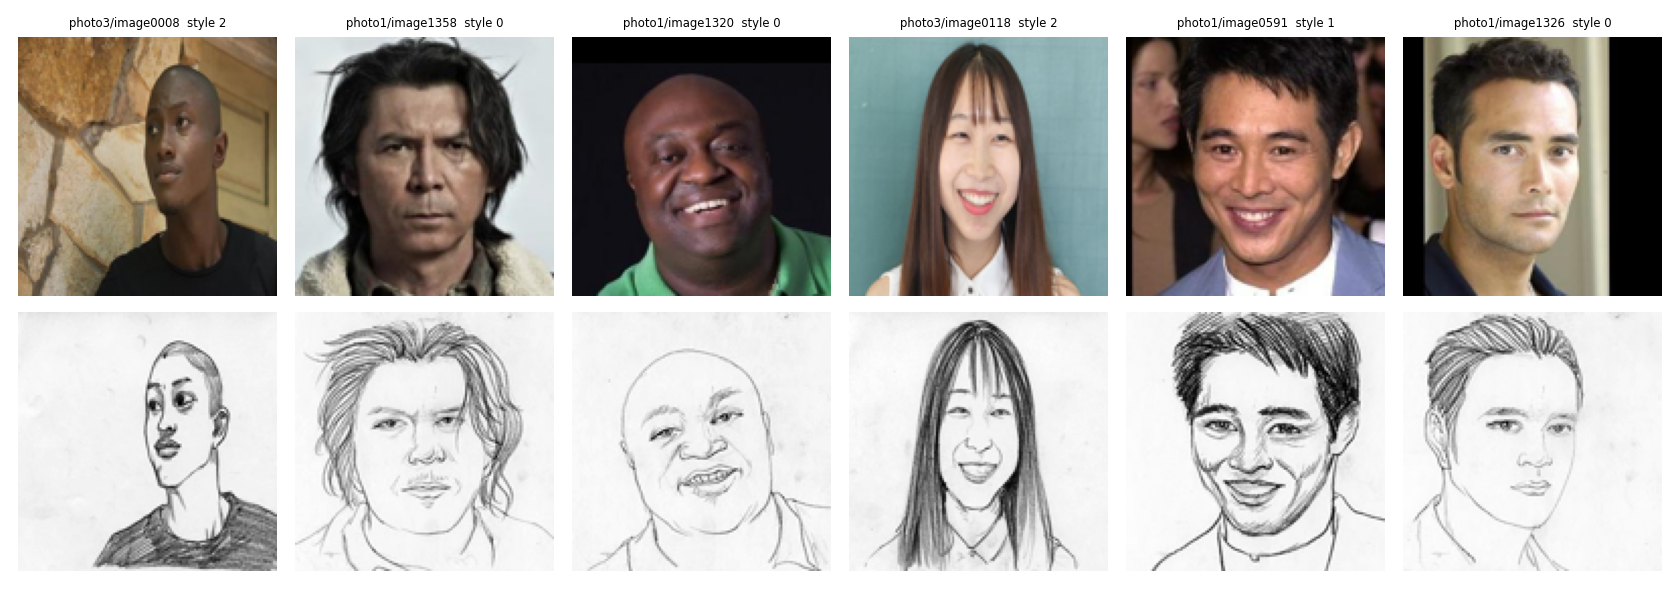
\includegraphics[width=\columnwidth]{t4_pairs_check.png}
\caption{Pairing check: six random FS2K training photos (top) with their ground-truth sketches (bottom) and style labels. Every pair is aligned, so paired training is valid.}
\label{fig:pairs}
\end{figure}

\subsection{Training protocol and tooling}
All models are PyTorch networks trained on a Kaggle GPU with AdamW~\cite{loshchilov2019} (autoencoders, classifier) or Adam with $\beta=(0.5,0.999)$ (GAN), cosine learning-rate decay, and seed 42. Every run logs hyper-parameters, losses, validation metrics, sample grids and checkpoints to MLflow (SQLite backend); Fig.~\ref{fig:mlflow} shows the tracking records of the Task~4 study and final run. Optuna uses the TPE sampler with a median pruner; trial budgets are short (6--20 epochs) and the winner is retrained for the full schedule. Because the Kaggle session was wiped once, every stage ends with a zipped download of its outputs. Models are exported to ONNX (opset 17) and compared with PyTorch on batch sizes 1, 8 and 64.

\begin{figure*}[t]
\centering
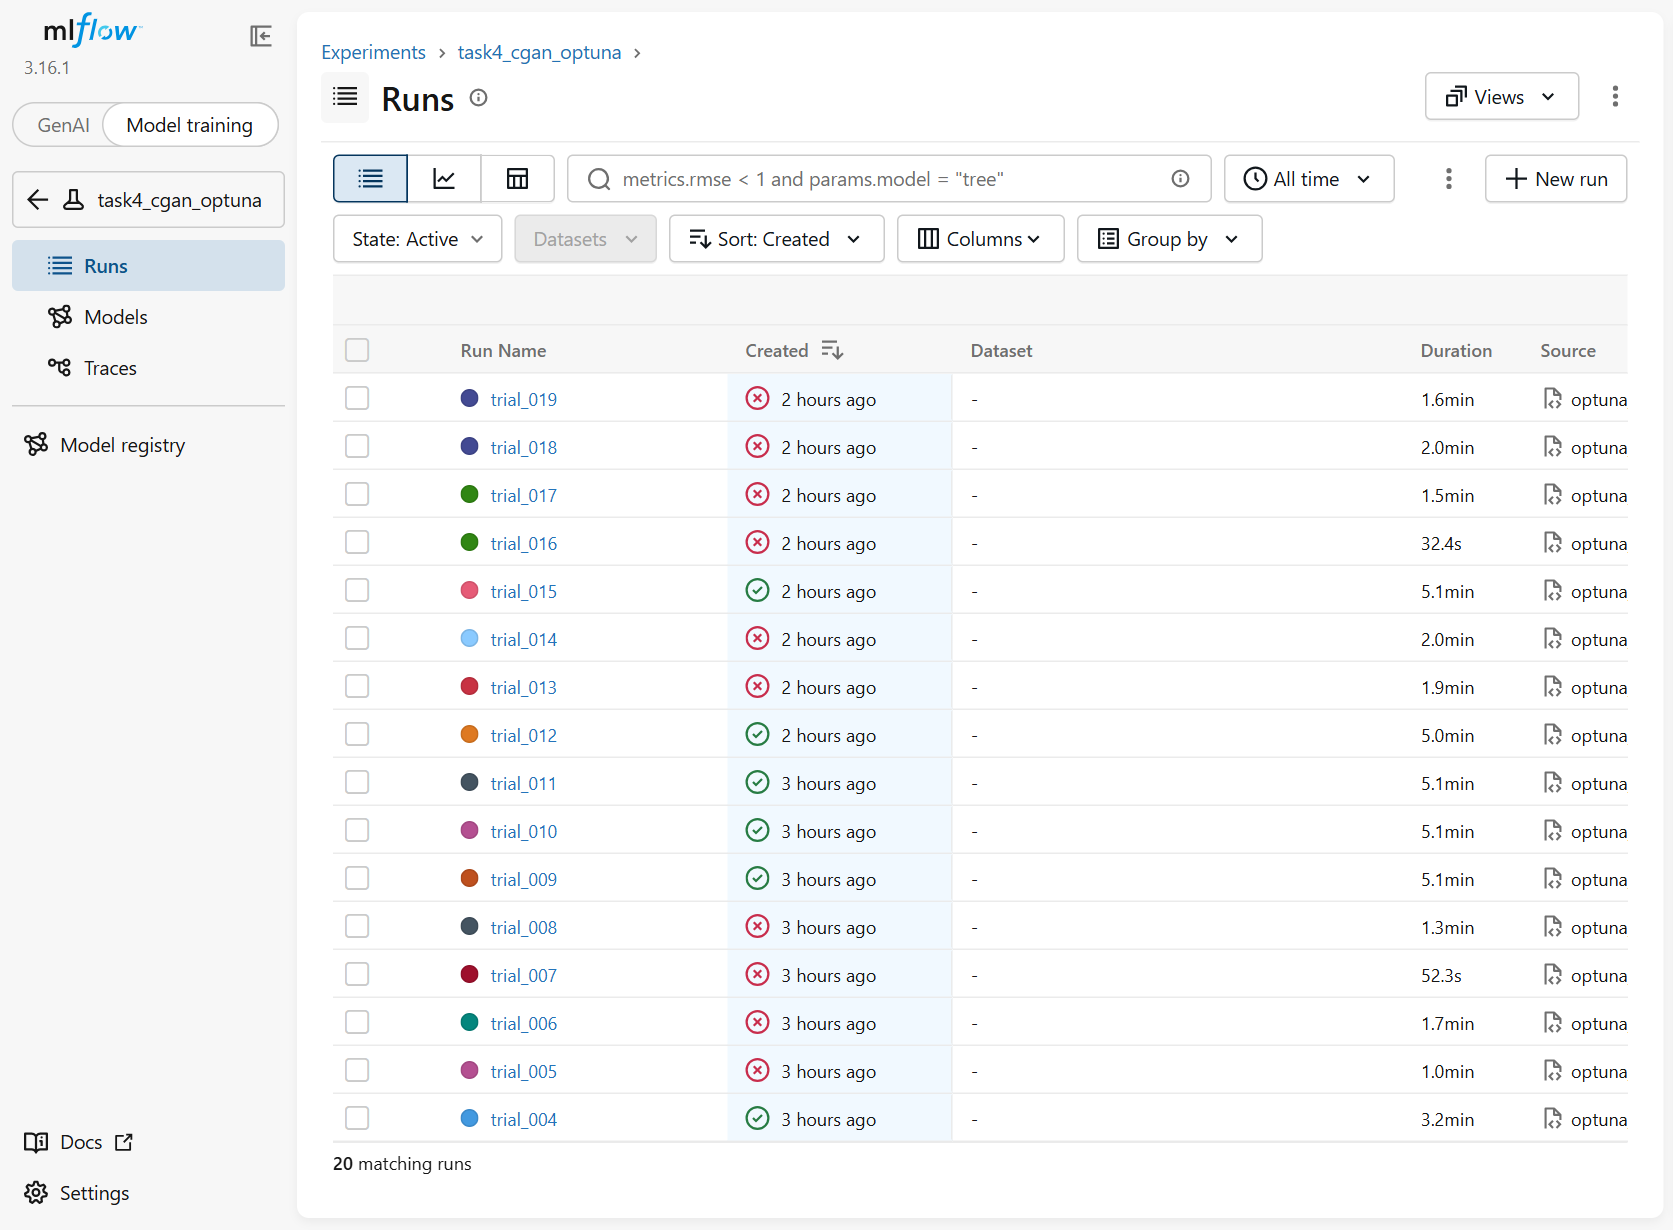
\includegraphics[width=0.49\textwidth]{mlflow_ui.png}\hfill
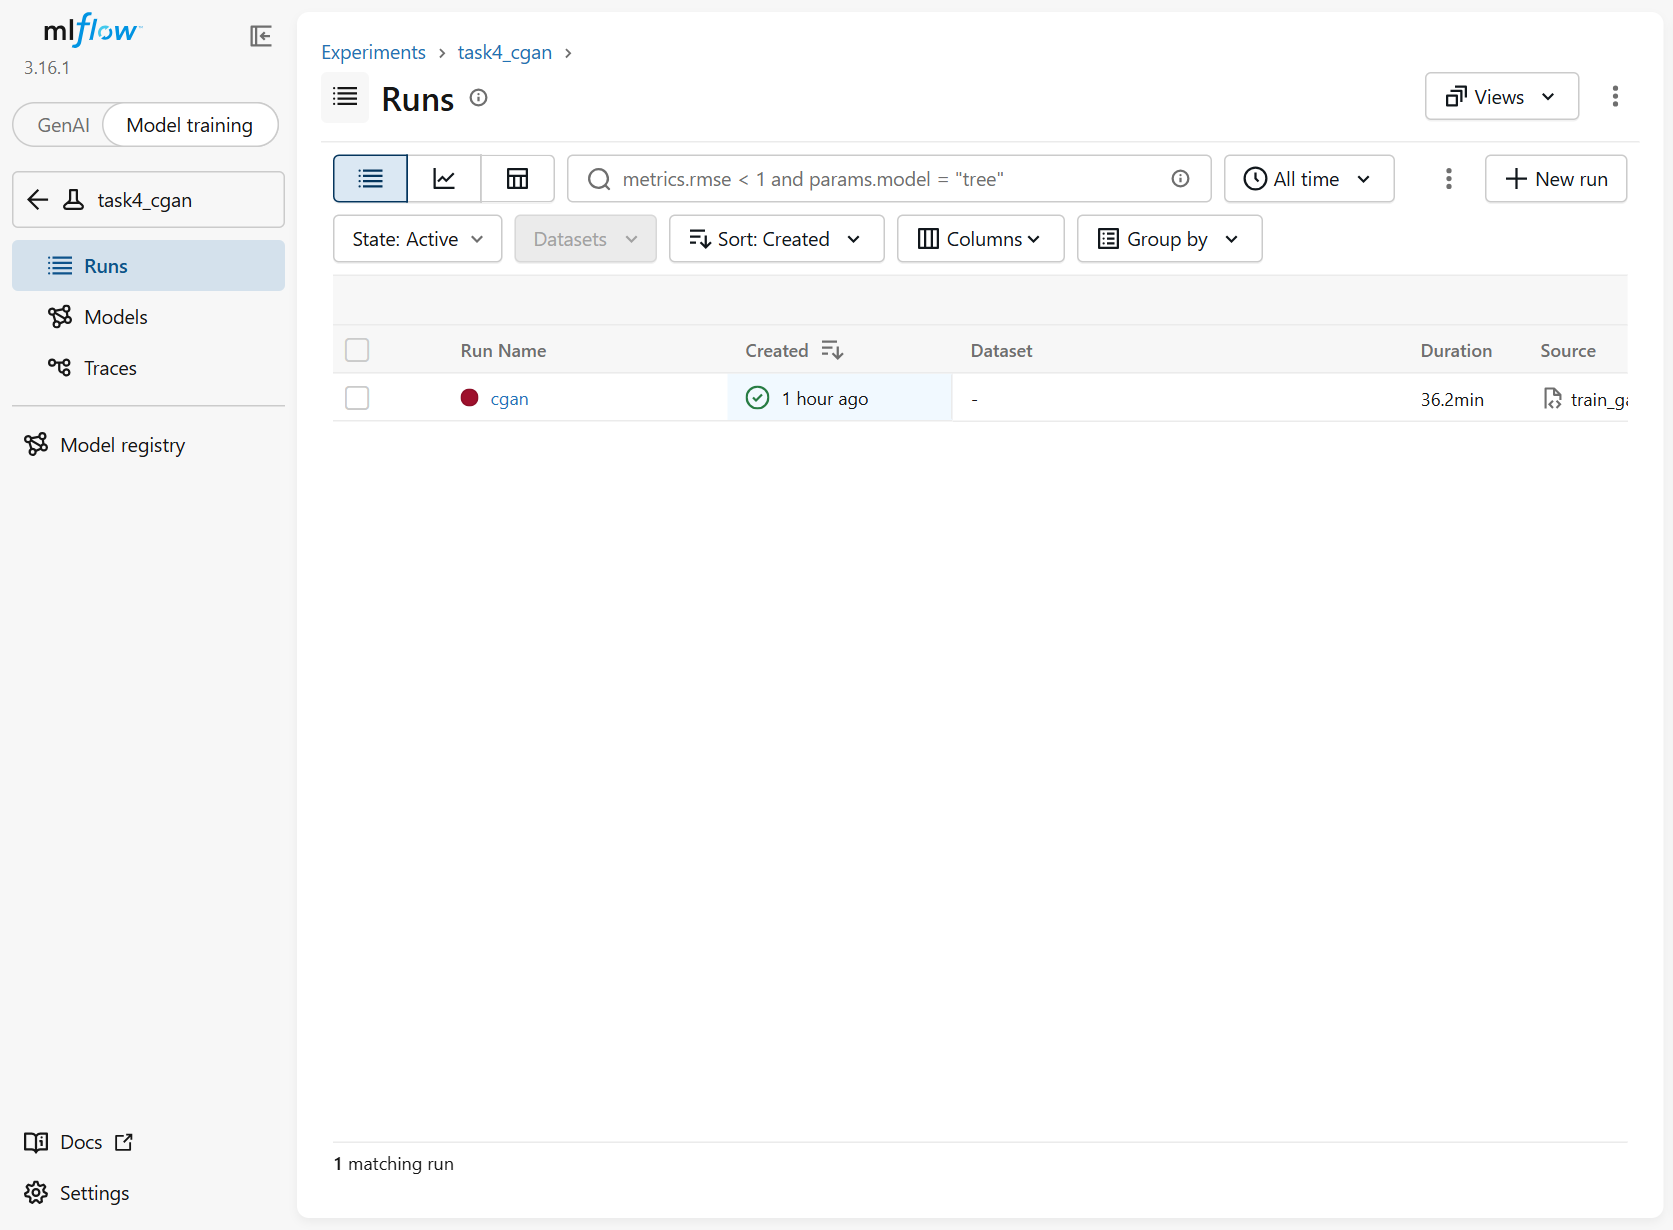
\includegraphics[width=0.49\textwidth]{mlflow_metrics.png}
\caption{Experiment tracking in MLflow. Left: the 20 runs of the Task~4 Optuna study (completed and pruned trials). Right: the separately logged loss components of the final cGAN run (D-real, D-fake, G-adversarial, G-$\ell_1$, validation D-fake) and the best validation score.}
\label{fig:mlflow}
\end{figure*}

\subsection{Hyper-parameter optimisation overview}
Table~\ref{tab:search} lists the search spaces and Table~\ref{tab:optuna} the outcomes. The objectives are always computed on the validation set only: $S=0.5\,\mathrm{SSIM}+0.5\min(\mathrm{PSNR},40)/40$ for the autoencoders and the MoE (independent of the loss weights, so trials with different $\alpha$ are comparable), macro-F1 for the classifier, and SSIM$-\ell_1$ for the GAN.

\begin{table*}[t]
\caption{Optuna search spaces (all studies: TPE sampler, seed 42, median pruner).}
\label{tab:search}
\centering\footnotesize
\begin{tabular}{@{}lp{14.2cm}@{}}
\toprule
Study & Search space\\
\midrule
T1 flat AE & lr $\log U[3\mathrm{e}{-4},3\mathrm{e}{-3}]$; batch $\{32,64,128\}$; latent $\{256,512,1024,2048,4096\}$; base channels $\{16,32,48\}$; dropout $U[0,0.3]$; $\alpha\sim U[0.5,0.95]$; 12 epochs/trial\\
T1 spatial AE & lr $\log U[1\mathrm{e}{-4},3\mathrm{e}{-3}]$; batch $\{32,64,128\}$; latent channels $\{8,16,32,64\}$ ($\times 8{\times}8$); base $\{16,32,48\}$; dropout $U[0,0.5]$; $\alpha\sim U[0.5,0.95]$; 12 epochs/trial\\
T2 classifier & lr $\log U[3\mathrm{e}{-4},5\mathrm{e}{-3}]$; batch $\{32,64,128\}$; channels \{small [16..128], medium [32..256], large [64..512]\}; dropout $U[0,0.5]$; weight decay $\log U[10^{-6},10^{-2}]$; 8 epochs/trial\\
T2 specialists (shared) & lr $\log U[1\mathrm{e}{-4},3\mathrm{e}{-3}]$; batch $\{32,64,128\}$; latent channels $\{16,32,64\}$; base $\{32,48,64\}$; $\alpha\sim U[0.5,0.95]$; 12 epochs/trial on a mixture of the three corruption types\\
T3 soft MoE & joint lr $\log U[2\mathrm{e}{-5},3\mathrm{e}{-4}]$; temperature $T\sim U[0.5,2]$; $\lambda_c\sim\log U[0.01,1]$; $\lambda_b\sim\log U[10^{-3},1]$; $\alpha\sim U[0.6,0.95]$; 6 epochs/trial (2 warm-up)\\
T4 cGAN & lr$_G$, lr$_D\sim\log U[5\mathrm{e}{-5},10^{-3}]$; batch $\{8,16,32\}$; base channels $\{32,48,64\}$; dropout $U[0,0.5]$; style dim $\{8,16,32,64\}$; $\lambda_{L1}\sim\log U[10,300]$; 20 epochs/trial\\
\bottomrule
\end{tabular}
\end{table*}

\begin{table*}[t]
\caption{Optuna outcomes. ``Score'' is the study objective of the best trial.}
\label{tab:optuna}
\centering\footnotesize
\begin{tabular}{@{}lrrrrl@{}}
\toprule
Study & Complete & Pruned & Best & Score & Selected configuration\\
\midrule
T1 flat AE & 14 & 10 & \#20 & 0.4240 & lr 3.6e-4, batch 32, latent 2048, base 32, dropout 0.287, $\alpha$ 0.903\\
T1 spatial AE & 18 & 6 & \#17 & 0.6137 & lr 1.08e-3, batch 32, latent ch 64, base 48, dropout 0.011, $\alpha$ 0.692\\
T2 classifier & 7 & 13 & \#4 & 1.0000 & lr 7.1e-4, batch 64, medium, dropout 0.455, wd 1.1e-5\\
T2 specialists & 11 & 9 & \#16 & 0.6202 & lr 6.5e-4, batch 32, latent ch 64, base 48, $\alpha$ 0.598\\
T3 soft MoE & 5 & 10 & \#8 & 0.8259 & lr 2.8e-5, $T$ 1.24, $\lambda_c$ 0.0117, $\lambda_b$ 0.535, $\alpha$ 0.691\\
T4 cGAN & 10 & 10 & \#9 & 0.4258 & lr$_G$ 5.8e-4, lr$_D$ 6.6e-4, batch 16, base 64, dropout 0.471, style dim 32, $\lambda_{L1}$ 272.5\\
\bottomrule
\end{tabular}
\end{table*}

\begin{table}[t]
\caption{fANOVA parameter importances (largest first; computed from few completed trials, so only indicative).}
\label{tab:importance}
\centering\footnotesize
\begin{tabular}{@{}lp{5.6cm}@{}}
\toprule
Study & Importances\\
\midrule
T1 flat & dropout .48, lr .46, $\alpha$ .05, latent .004, base .003, batch .000\\
T1 spatial & lr .69, latent ch .15, $\alpha$ .12, dropout .03, base .01, batch .01\\
T2 classifier & channels .42, lr .40, wd .10, batch .05, dropout .03\\
T2 specialists & $\alpha$ .58, lr .38, latent ch .02, batch .01, base .01\\
T3 soft MoE & $\lambda_c$ .35, $\lambda_b$ .27, $T$ .23, lr .08, $\alpha$ .08\\
T4 cGAN & lr$_G$ .32, dropout .28, lr$_D$ .23, $\lambda_{L1}$ .17, others $\approx$0\\
\bottomrule
\end{tabular}
\end{table}

% =====================================================================
\section{Task 1: Universal Multi-Corruption Denoising Autoencoder}
\subsection{Architecture and the bottleneck investigation}
\textbf{First design (flat bottleneck).} Five stages of stride-2 and stride-1 convolutions (BatchNorm, LeakyReLU) reduce $128{\times}128{\times}3$ to $4{\times}4{\times}256$; a linear layer maps this to a latent vector $z\in\mathbb{R}^{256}$ with dropout, and a mirrored decoder (nearest-neighbour up-sampling followed by convolutions, sigmoid output) reconstructs the image. There are no skip connections, so all information passes through $z$ (Fig.~\ref{fig:t1arch}a).

\textbf{Observation.} After 60 epochs this model reached a validation PSNR of only 18.0\,dB, almost independent of the input condition (Table~\ref{tab:ablation}); clean images came out at 18.1\,dB although they entered at the capped 50\,dB. Train and validation losses were close, so the model underfitted. Optuna over latent sizes 256--4096 improved it by only 0.8\,dB, and the latent size had an importance of just 0.004. We concluded that the limit was not the number of latent values but the flatten + fully connected bottleneck, which discards spatial layout.

\textbf{Final design (spatial bottleneck).} Four stride-2 stages reduce the image to $8{\times}8{\times}8b$ ($b$ = base channels); a $1{\times}1$ convolution produces the bottleneck $8{\times}8{\times}C_z$ (with $C_z=64$: 4\,096 values, a $12\times$ compression of the 49\,152 input values), and a mirrored decoder reconstructs the image (Fig.~\ref{fig:t1arch}b). It is still a genuine compressing autoencoder without skip connections, but it keeps \emph{where} content is located. We did not use skip connections; a limited-skip ablation is future work.

\begin{figure*}[t]
\centering
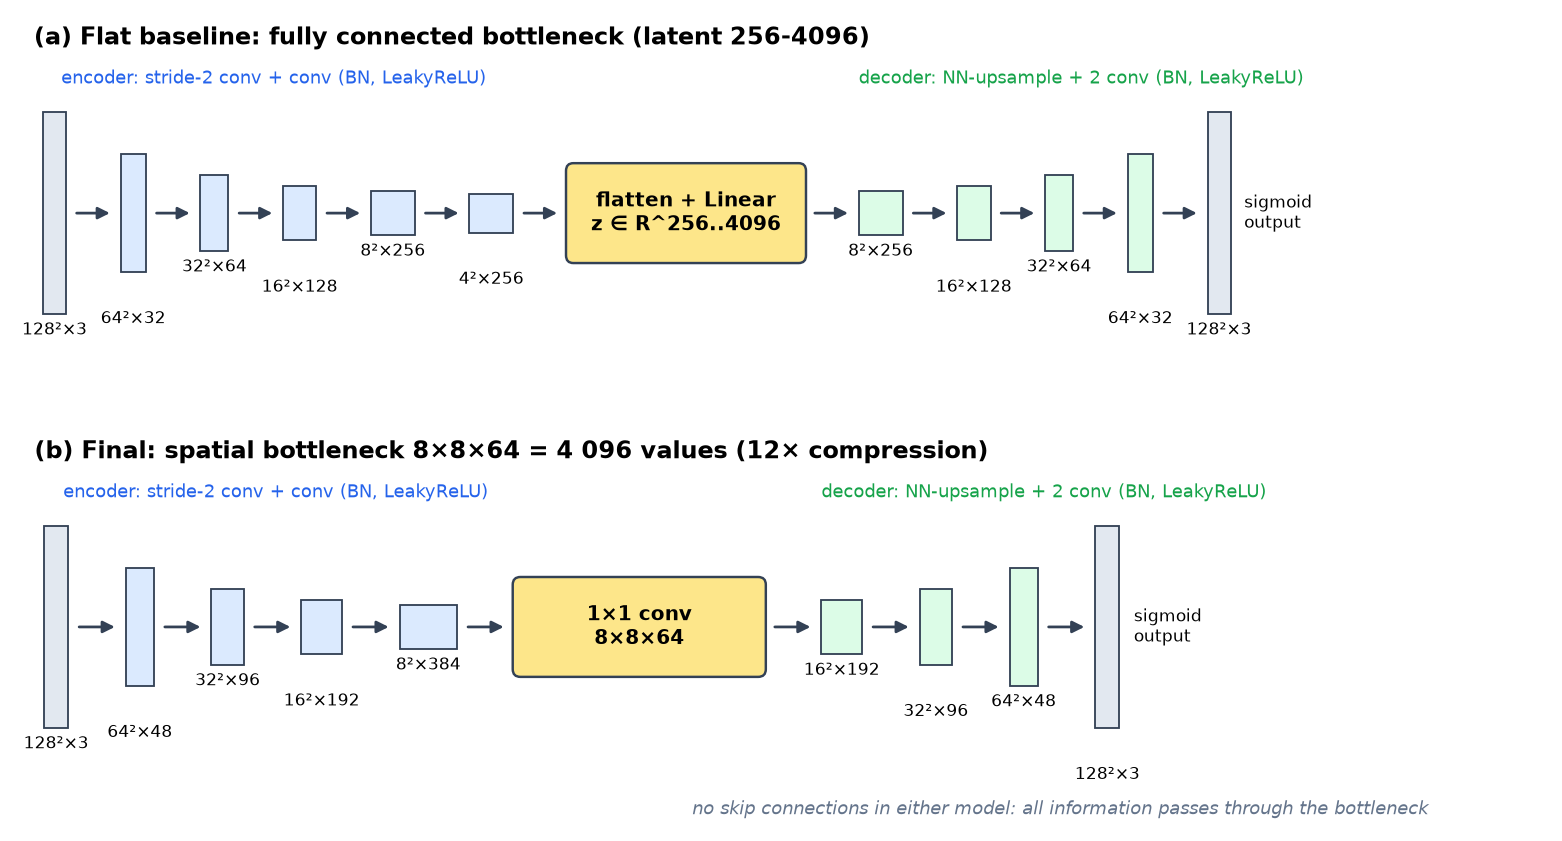
\includegraphics[width=0.86\textwidth]{t1_arch.png}
\caption{Task 1 autoencoders. (a) Flat baseline with a fully connected latent vector. (b) Final model with a convolutional $8{\times}8{\times}64$ bottleneck ($b=48$). Neither model has skip connections.}
\label{fig:t1arch}
\end{figure*}

\begin{table}[t]
\caption{Bottleneck ablation on the validation manifest (all 736 images, sampled severities).}
\label{tab:ablation}
\centering\footnotesize
\begin{tabular}{@{}lrrrr@{}}
\toprule
Model & Epochs & PSNR & SSIM & Score\\
\midrule
Flat, 256-d (baseline) & 60 & 18.0 & 0.418 & 0.435\\
Flat, 2048-d (Optuna) & 80 & 18.8 & 0.439 & 0.455\\
Spatial $8{\times}8{\times}64$ & 80 & \textbf{25.8} & \textbf{0.801} & \textbf{0.723}\\
\bottomrule
\end{tabular}
\end{table}

\subsection{Loss, training and optimisation}
With clean target $x$, corrupted input $\tilde x$, encoder $E$ and decoder $D$, $\hat x=D(E(\tilde x))$ and
\begin{equation}
\mathcal{L}_{AE}=\alpha\,\lVert x-\hat x\rVert_1+(1-\alpha)\bigl(1-\mathrm{SSIM}(x,\hat x)\bigr).
\end{equation}
$\alpha=0.8$ was the suggested start; Optuna selected $\alpha=0.692$ for the final model. Training used runtime corruptions, AdamW (weight decay $10^{-4}$), cosine decay and 80 epochs, with the checkpoint chosen by the validation score $S$. The search spaces and results are in Tables~\ref{tab:search}--\ref{tab:importance} and Fig.~\ref{fig:t1optuna}. For the spatial model the learning rate dominates (importance 0.69) and both $C_z=64$ and $b=48$ lie at the upper end of their ranges, so slightly larger values might help (a limitation). Fig.~\ref{fig:t1curves} shows that the spatial model passes the flat model's final score within its first few epochs and keeps improving for the whole schedule, with training and validation losses close together.

\begin{figure*}[t]
\centering
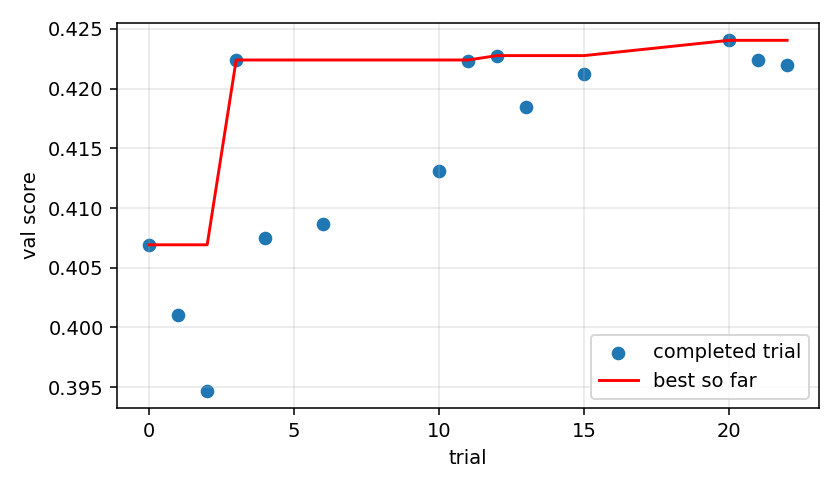
\includegraphics[width=0.245\textwidth]{t1_optuna_flat_history.png}\hfill
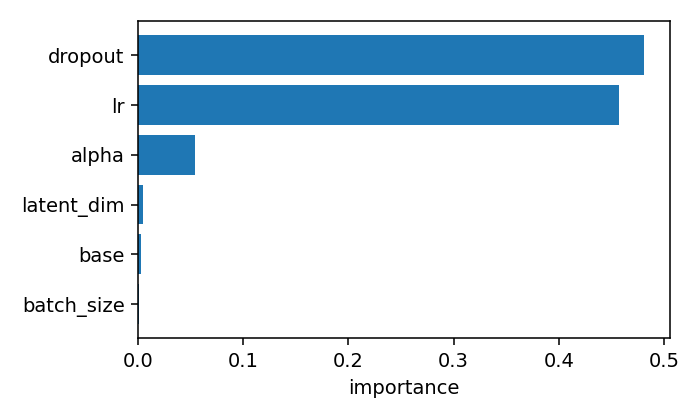
\includegraphics[width=0.21\textwidth]{t1_optuna_flat_importance.png}\hfill
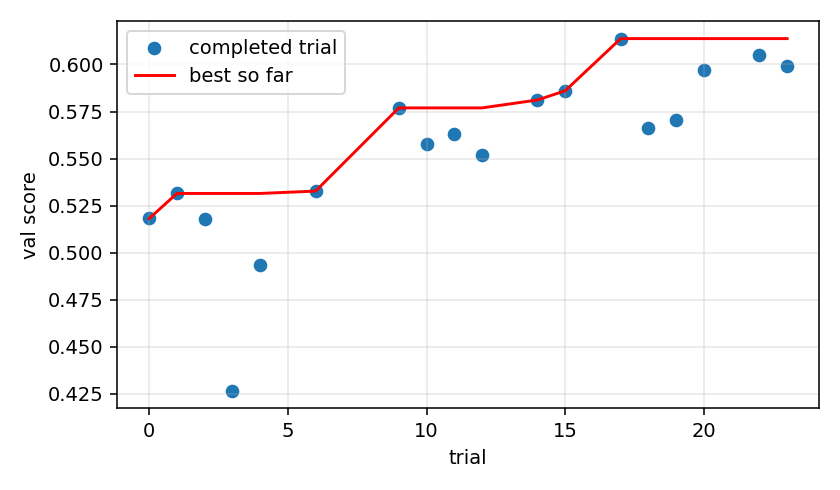
\includegraphics[width=0.245\textwidth]{t1_optuna_spatial_history.png}\hfill
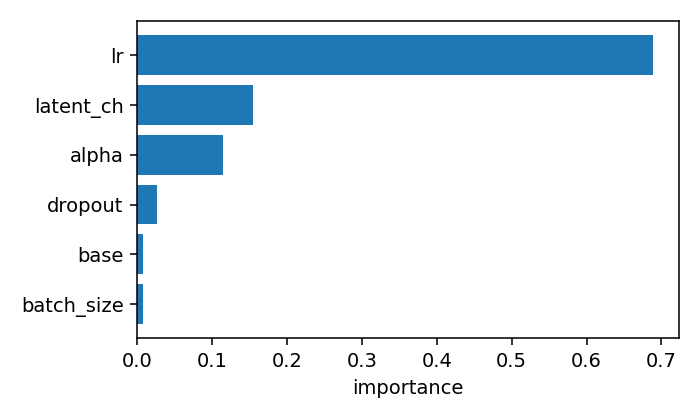
\includegraphics[width=0.21\textwidth]{t1_optuna_spatial_importance.png}
\caption{Task 1 Optuna results: flat study (left two) and spatial study (right two), optimisation history and fANOVA parameter importance. The best spatial trial (0.614) is far above the best flat trial (0.424) for the same 12-epoch budget.}
\label{fig:t1optuna}
\end{figure*}

\begin{figure}[t]
\centering
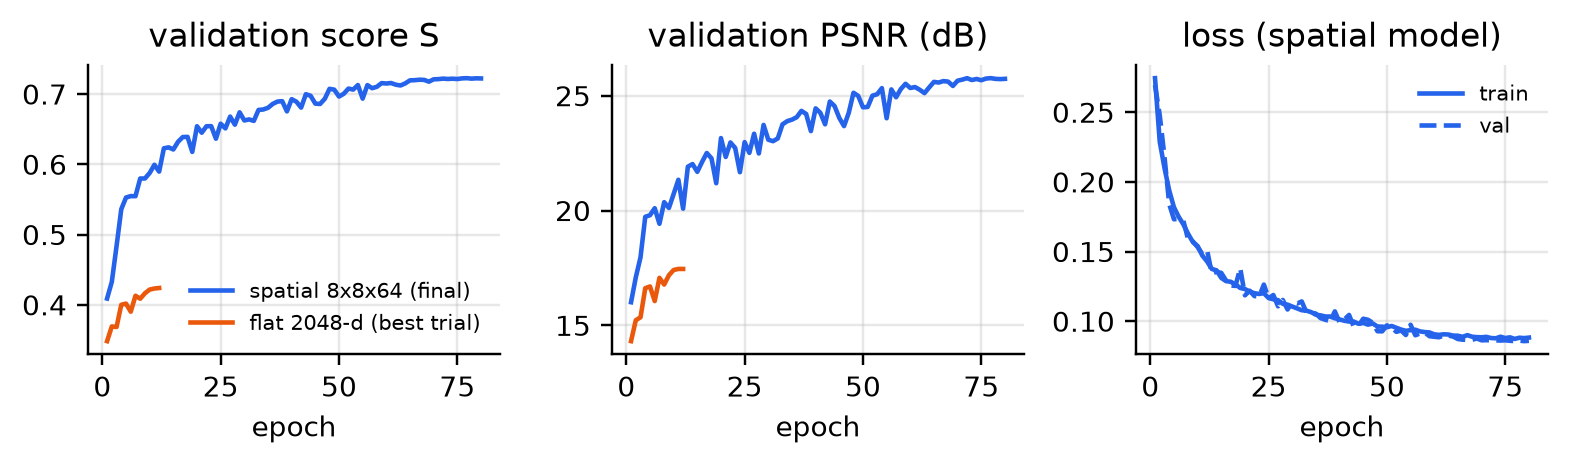
\includegraphics[width=\columnwidth]{t1_curves.png}
\caption{Task 1 training curves: the final spatial model (80 epochs) against the best flat Optuna trial (12 epochs): validation score, validation PSNR and the spatial model's training and validation loss.}
\label{fig:t1curves}
\end{figure}

\subsection{Results}
Table~\ref{tab:t1type} reports the official test set by corruption type and Table~\ref{tab:t1sev} by severity. The validation results agree within 0.4\,dB, so the model was not tuned to the validation set. PSNR of clean images is capped at 50\,dB because a perfect copy has infinite PSNR.

\begin{table}[t]
\caption{Task 1, test set by corruption type (PSNR in dB). ``In'' = corrupted input, ``Out'' = restored.}
\label{tab:t1type}
\centering\footnotesize
\begin{tabular}{@{}lrrrrr@{}}
\toprule
Type & $n$ & PSNR in & PSNR out & SSIM in & SSIM out\\
\midrule
Salt-and-pepper & 11\,007 & 16.39 & 26.61 & 0.382 & 0.818\\
Blur & 11\,007 & 27.78 & 26.37 & 0.812 & 0.798\\
Occlusion & 11\,007 & 13.57 & 22.08 & 0.709 & 0.724\\
Clean & 3\,669 & 50.00 & 26.88 & 1.000 & 0.831\\
\bottomrule
\end{tabular}
\end{table}

\begin{table}[t]
\caption{Task 1, test set by corruption type and severity (3\,669 images each).}
\label{tab:t1sev}
\centering\footnotesize
\begin{tabular}{@{}llrrrr@{}}
\toprule
Type & Severity & PSNR in & PSNR out & SSIM in & SSIM out\\
\midrule
\multirow{3}{*}{Salt-and-pepper} & low & 20.14 & 26.84 & 0.603 & 0.829\\
 & medium & 15.88 & 26.68 & 0.340 & 0.821\\
 & high & 13.14 & 26.31 & 0.204 & 0.805\\
\midrule
\multirow{3}{*}{Blur} & low & 32.27 & 27.03 & 0.943 & 0.830\\
 & medium & 26.73 & 26.82 & 0.804 & 0.820\\
 & high & 24.33 & 25.27 & 0.690 & 0.746\\
\midrule
\multirow{3}{*}{Occlusion} & low & 16.68 & 23.97 & 0.862 & 0.782\\
 & medium & 13.27 & 22.16 & 0.726 & 0.733\\
 & high & 10.76 & 20.10 & 0.539 & 0.657\\
\bottomrule
\end{tabular}
\end{table}

\textbf{Interpretation.} Salt-and-pepper restoration is almost independent of severity (26.8$\to$26.3\,dB), so the network treats this noise as easy to remove: at $p=0.15$ it gains 13\,dB. Occlusion degrades steadily with the covered area because more content must be invented. Blur is the failure of this model: at low severity restoration \emph{reduces} quality (32.3$\to$27.0\,dB) because the bottleneck imposes a $\approx$27\,dB ceiling that is below what a mildly blurred input already offers; only at high severity does it help. The same ceiling explains the clean row. This directly motivates the identity bypass of Task 2.

\subsection{Visual results and failure cases}
Fig.~\ref{fig:t1vis} shows twelve representative test examples (four per corruption) with absolute-error maps, and the four lowest-SSIM test cases. Salt-and-pepper restorations are visually clean with errors confined to edges; blurred inputs are partially sharpened (e.g.\ the whiskers and eyes of the cats); occlusion fills are smooth and plausible in colour but lack texture.

The failures fall into three types. (1) \emph{Holes on a uniform dark background}: two of the four worst test cases are the same cat on a black background with medium and high occlusion (SSIM 0.28 and 0.36). The network fills the holes, and even parts of the untouched black background, with a bright grey-brown blur, i.e.\ it predicts the average colour of pet photographs rather than the local context. (2) \emph{Large boxes on the subject}: with three boxes on a dog in a flower field (SSIM 0.36) the silhouette is lost and replaced by a smooth patch; the four worst \emph{validation} cases (SSIM 0.42--0.50) are all of this kind, e.g.\ a box covering a white dog. Both are the expected consequence of regression losses ($\ell_1$/SSIM), which return the mean of the plausible completions. (3) \emph{Fine texture under heavy blur}: the same flower-field image at blur $(7,2.5)$ (SSIM 0.38) cannot be restored because the high-frequency detail lies above the $\approx$27\,dB capacity of the bottleneck.

\begin{figure*}[t]
\centering
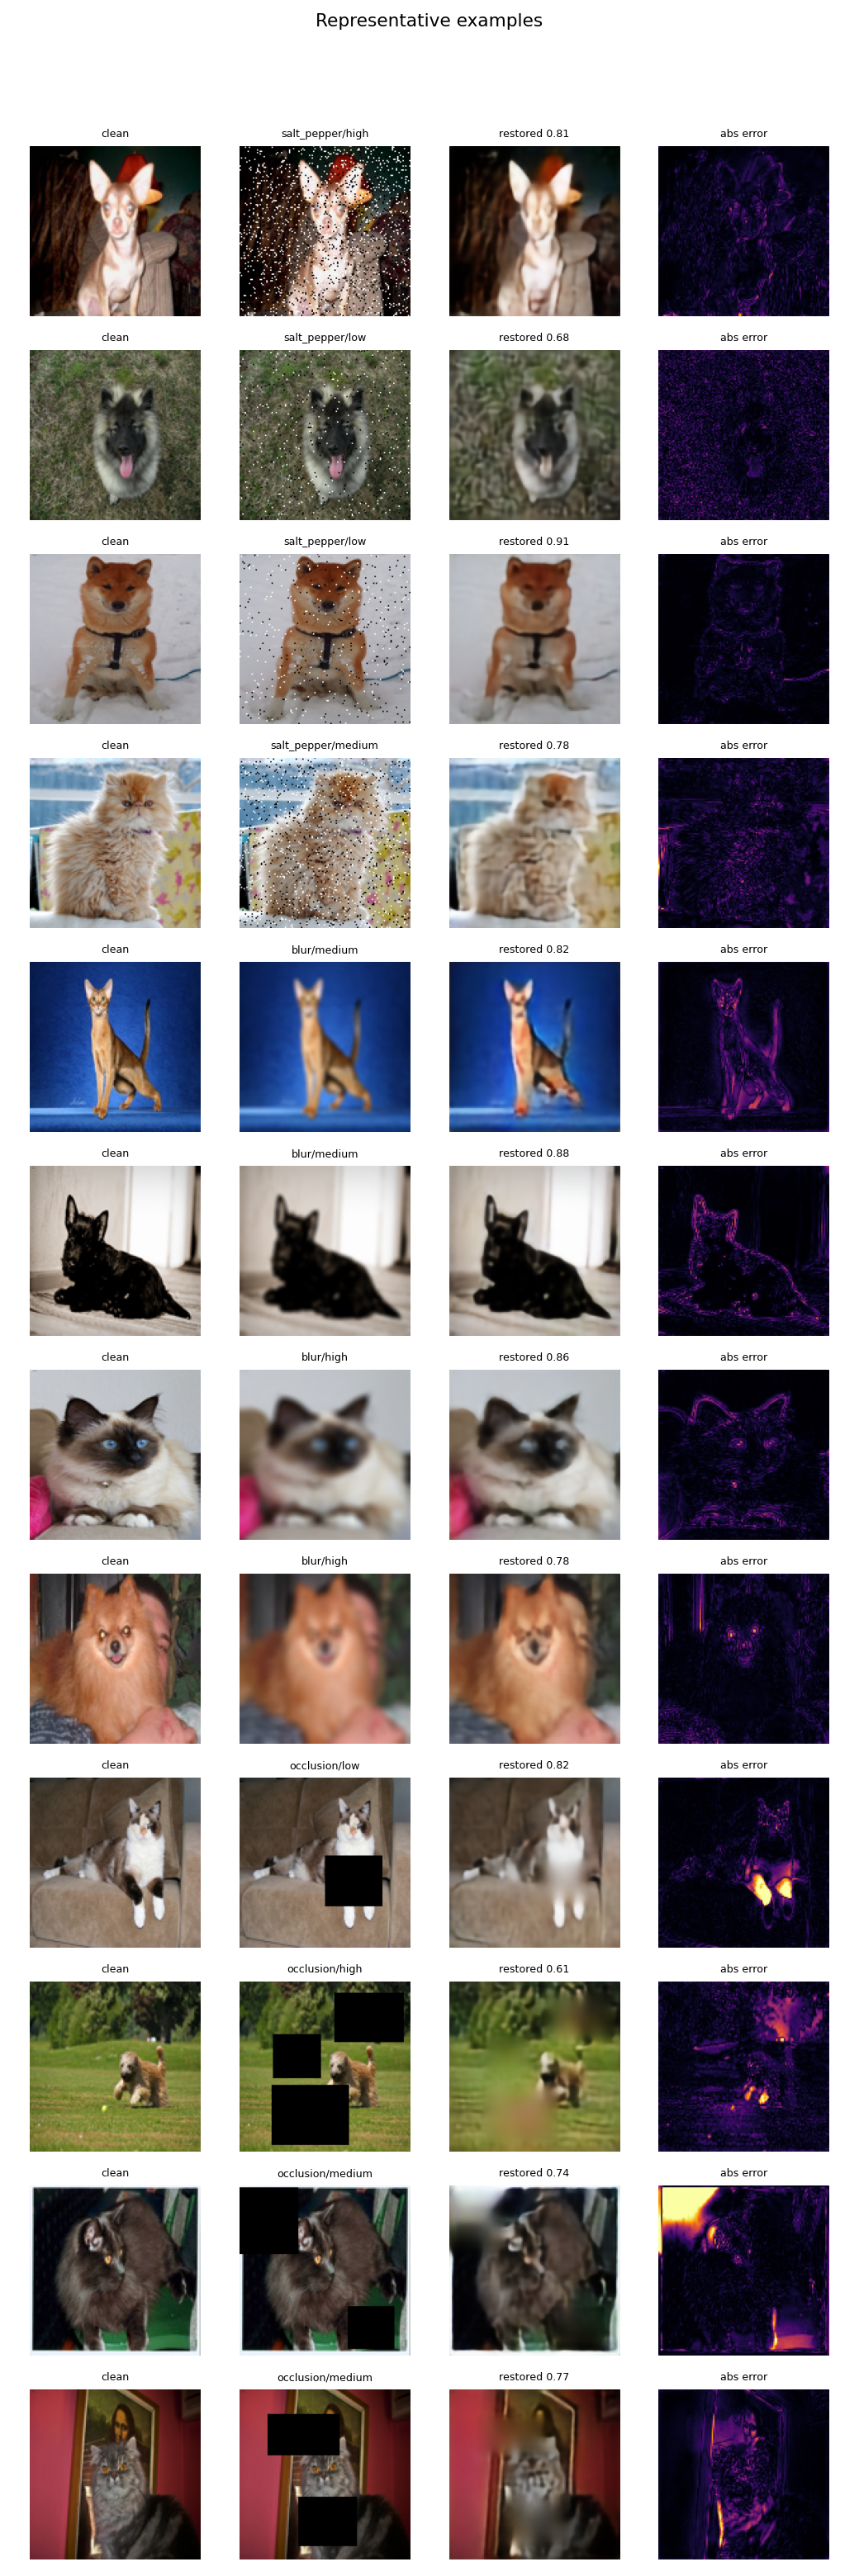
\includegraphics[height=0.47\textheight]{t1_test_examples.png}\hspace{6mm}
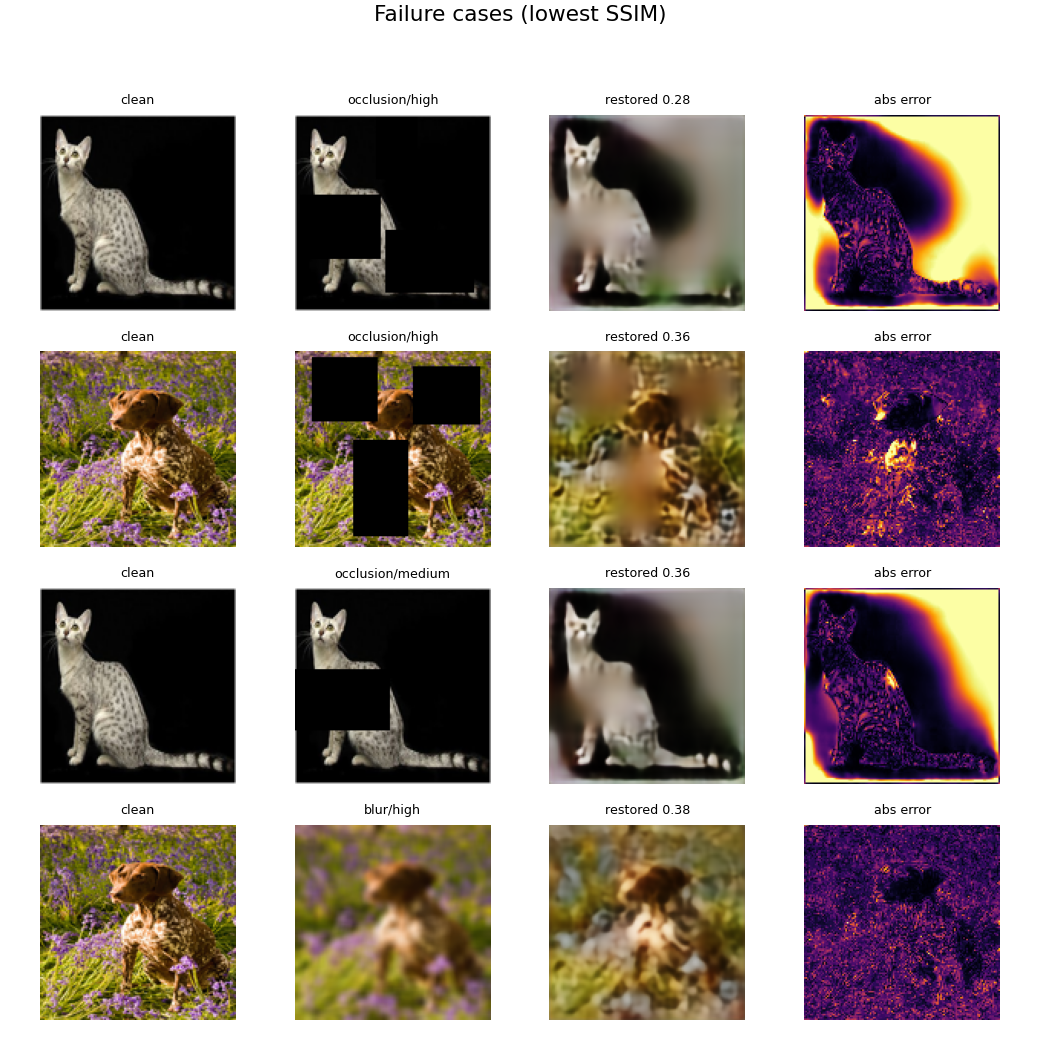
\includegraphics[height=0.24\textheight]{t1_test_failures.png}
\caption{Task 1 on the official test set. Left: twelve representative examples (clean target, corrupted input, restored output with SSIM, absolute error). Right: the four lowest-SSIM failure cases.}
\label{fig:t1vis}
\end{figure*}

\subsection{Export}
The final model is exported to ONNX (26.6\,MB, input \texttt{input}, output \texttt{restored}, dynamic batch). The maximum absolute difference to PyTorch is $1.7\times10^{-6}$ and a $128{\times}128$ image takes 42\,ms on a CPU (Table~\ref{tab:onnx}).

% =====================================================================
\section{Task 2: Corruption Classifier and Hard-Routed Specialists}
\subsection{Corruption classifier}
\textbf{Architecture.} Four stages of two $3{\times}3$ convolutions (BatchNorm, LeakyReLU) and max-pooling, followed by global average pooling, dropout and a linear 4-way head. There is deliberately no early down-sampling: salt-and-pepper noise and mild blur are pixel-level cues that strided stems would hide.

\textbf{Balanced batches.} The labels come from the runtime corruption pipeline. A custom sampler places exactly $B/4$ samples of every class in every batch, which is stricter than balance on average. The loss is multiclass cross-entropy,
\begin{equation}
\mathcal{L}_{CE}=-\sum_c y_c\log p_c,\qquad \hat k=\arg\max_c p_c.
\end{equation}

\textbf{Optimisation.} The study (Tables~\ref{tab:search}--\ref{tab:optuna}) tuned learning rate, batch size, channel configuration, dropout and weight decay against validation macro-F1. The objective saturated: trials \#4 and \#16 both reached 1.0000 and most others 0.9987, so the study could not rank configurations and the choice of trial \#4 is partly arbitrary; the importances in Table~\ref{tab:importance} are therefore weak evidence. The selected model (medium channels) was trained for 30 epochs.

\textbf{Results.} Validation accuracy is 100\% (736 images). On the test set (Table~\ref{tab:clf}, Fig.~\ref{fig:confusion}) accuracy is 99.78\% with macro precision/recall/F1 of 0.9956/0.9972/0.9964. All 80 errors (0.218\%) fall in two places: 58 low-severity occlusions (one box covering about 10\% of the image) predicted as clean, and 22 clean images predicted as blur (15) or occlusion (7). Blur and salt-and-pepper are classified perfectly at all severities, including blur $(3,0.7)$ and $p=0.03$, contrary to our expectation that mild blur would be the hard case.

\begin{table}[t]
\caption{Classifier, test set, per class (normalised confusion matrix in Fig.~\ref{fig:confusion}).}
\label{tab:clf}
\centering\footnotesize
\begin{tabular}{@{}lrrrr@{}}
\toprule
Class & Precision & Recall & F1 & Support\\
\midrule
Clean & 0.9843 & 0.9940 & 0.9892 & 3\,669\\
Salt-and-pepper & 1.0000 & 1.0000 & 1.0000 & 11\,007\\
Blur & 0.9986 & 1.0000 & 0.9993 & 11\,007\\
Occlusion & 0.9994 & 0.9947 & 0.9970 & 11\,007\\
\midrule
Macro average & 0.9956 & 0.9972 & 0.9964 & 36\,690\\
\bottomrule
\end{tabular}
\end{table}

\begin{figure}[t]
\centering
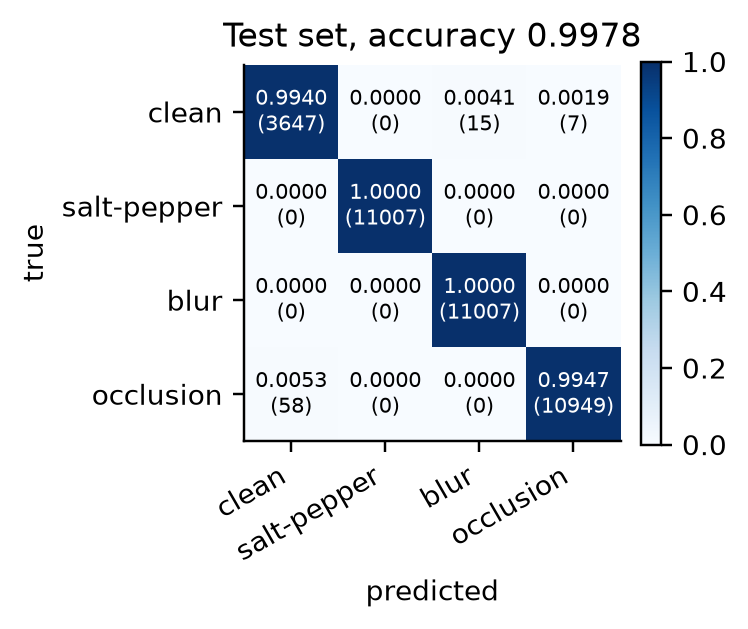
\includegraphics[width=0.82\columnwidth]{t2_confusion_test.png}
\caption{Normalised four-class confusion matrix of the corruption classifier on the official test set (counts in parentheses).}
\label{fig:confusion}
\end{figure}

\subsection{Specialist autoencoders}
Three specialists use the spatial autoencoder of Task~1 with independent parameters (seeds 42, 43, 44), each trained only on its own corruption with the clean image as target. Following the permitted shortcut, one shared Optuna search found a common architecture: each trial trains a single model on the mixture of the three corruptions (clean images excluded, since they bypass the experts), tuning learning rate, batch size, bottleneck channels, base channels and the $\ell_1$/SSIM weight (Table~\ref{tab:search}). The winner (latent channels 64, base 48, $\alpha=0.598$, lr $6.5\times10^{-4}$) was then trained three times for 60 epochs (Table~\ref{tab:spec}). Again $C_z=64$ sits at the top of its range.

\begin{table}[t]
\caption{Specialists on the validation manifest (final epoch; best-score epoch reported in the last column).}
\label{tab:spec}
\centering\footnotesize
\begin{tabular}{@{}lrrrr@{}}
\toprule
Specialist & Val samples & PSNR & SSIM & Best score\\
\midrule
Salt-and-pepper & 178 & 27.27 & 0.846 & 0.7638\\
Blur & 180 & 27.07 & 0.833 & 0.7567\\
Occlusion & 181 & 22.21 & 0.730 & 0.6429\\
\bottomrule
\end{tabular}
\end{table}

\subsection{Hard-routed inference}
Inference is
\begin{equation}
\hat x=\begin{cases}\tilde x, & \hat k=\text{clean (identity bypass)}\\ E_{\hat k}(\tilde x), & \hat k\in\{\text{salt, blur, occlusion}\}\end{cases}
\end{equation}
so a clean-looking image is never processed by an expert. The system was evaluated twice: with \emph{oracle} routing (the known label of the test manifest selects the expert, showing the specialists' ability) and with \emph{predicted} routing (the classifier selects the expert, showing the operational system). Table~\ref{tab:t2type} gives the test results.

\begin{table}[t]
\caption{Task 2, test set by type: universal model versus hard routing with oracle and predicted routes (PSNR dB / SSIM).}
\label{tab:t2type}
\centering\footnotesize
\setlength{\tabcolsep}{4pt}
\begin{tabular}{@{}lrrrrr@{}}
\toprule
 & \multicolumn{3}{c}{PSNR} & \multicolumn{2}{c}{SSIM}\\
\cmidrule(lr){2-4}\cmidrule(l){5-6}
Type & Univ. & Oracle & Pred. & Univ. & Pred.\\
\midrule
Salt-and-pepper & 26.61 & 27.07 & 27.07 & 0.818 & 0.842\\
Blur & 26.37 & 26.62 & 26.62 & 0.798 & 0.814\\
Occlusion & 22.08 & 22.22 & 22.22 & 0.724 & 0.730\\
Clean & 26.89 & 50.00 & 49.86 & 0.831 & 0.999\\
\midrule
Corrupted-only mean & 25.02 & 25.30 & 25.30 & 0.780 & 0.795\\
\bottomrule
\end{tabular}
\end{table}

\textbf{Findings.} (1) Specialisation helps only slightly: 0.14--0.46\,dB over the universal model, which is small relative to the noise of a 180-image validation set per type; the shared $\approx$27\,dB bottleneck ceiling limits both. (2) The large benefit of hard routing is the identity bypass: clean images stay exact (SSIM 0.999 against 0.831). (3) Predicted routing is as good as oracle routing on average (25.30\,dB for both on corrupted inputs): there were no routing errors on validation (0/736), and on the test set 80 of 36\,690 samples (0.218\%) are misrouted (Table~\ref{tab:routefail}).

\begin{table}[t]
\caption{Routing errors on the test set and their cost (PSNR loss = oracle minus predicted).}
\label{tab:routefail}
\centering\footnotesize
\begin{tabular}{@{}llrrr@{}}
\toprule
True & Routed to & $n$ & Mean conf. & PSNR loss\\
\midrule
Clean & blur expert & 15 & 0.78 & 20.0\,dB\\
Clean & occlusion expert & 7 & 0.80 & 28.5\,dB\\
Occlusion (low) & clean (bypass) & 58 & 0.76 & $-0.4$\,dB\\
\bottomrule
\end{tabular}
\end{table}

\textbf{Failure analysis.} The two types of routing failure have opposite consequences. \emph{Clean images sent to an expert} are softened: the apparent loss of 20--28\,dB is partly an artefact of the 50\,dB cap on the perfect copy, but the real effect is that a pristine image comes back at about 30\,dB (blur expert) or 22\,dB (occlusion expert). Fig.~\ref{fig:routefail} shows the six most costly cases and explains them: four are photographs with black letterbox bars or a large uniform black background, which the classifier mistakes for occlusion boxes, and one is a soft-focus photograph of a long-haired dog that genuinely looks blurred. The occlusion expert then ``repairs'' the black bars by painting a bright, smeared border into the image. \emph{The 58 missed occlusions cost nothing}; predicted routing is even 0.4\,dB better than oracle routing there, because the specialist slightly degrades these images. The data confirm why they are missed: their corrupted input already has a mean PSNR of 24.8\,dB against the clean image, compared with 16.6\,dB for the correctly detected low-severity occlusions, i.e.\ the single small box lies on a region that was already dark, so it barely changes the image. All mistakes have low confidence (0.76--0.80), which suggests that a confidence threshold or a soft gate could avoid them.

\begin{figure}[t]
\centering
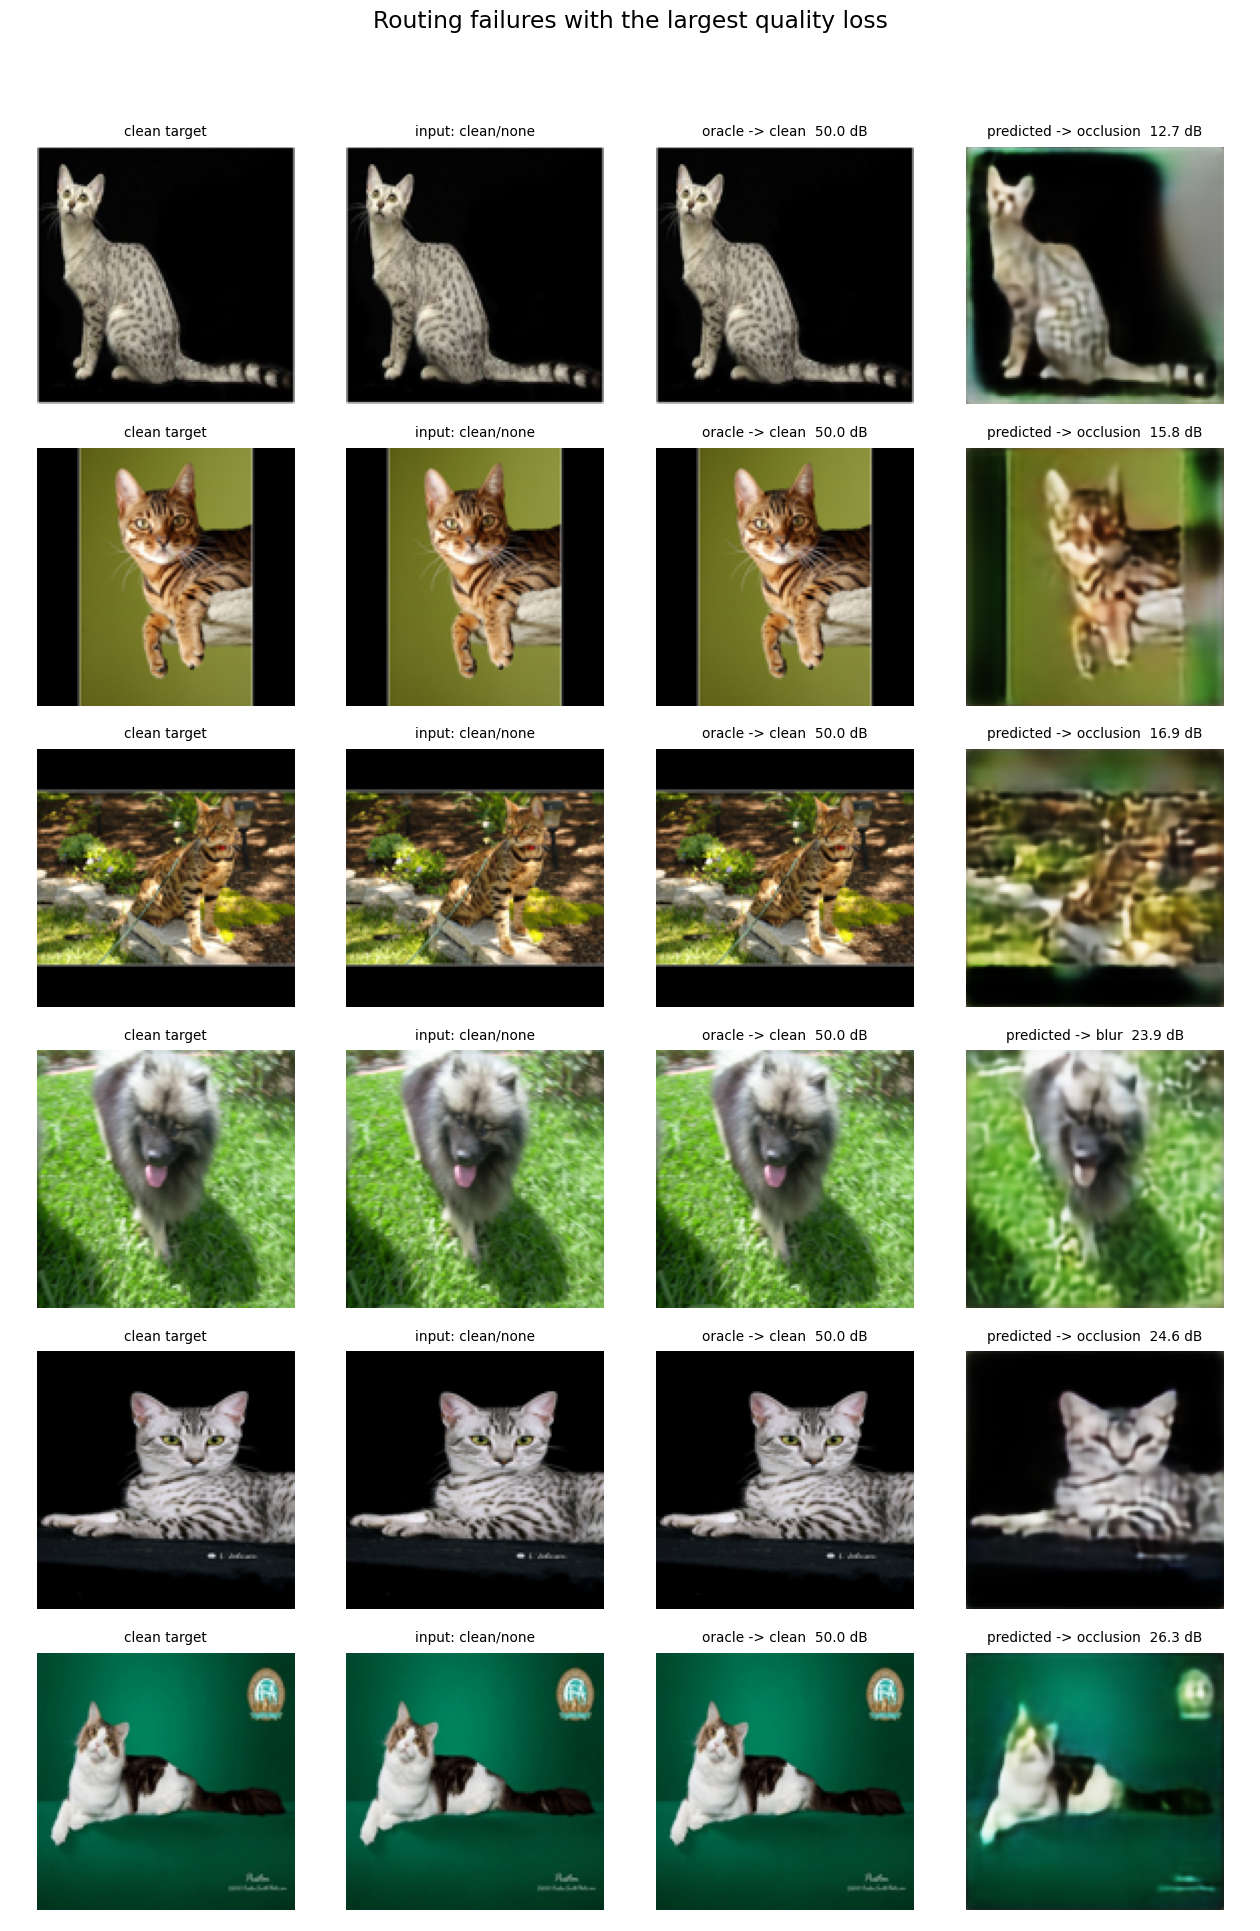
\includegraphics[width=0.92\columnwidth]{t2_routing_failures.png}
\caption{The six test routing failures with the largest quality loss (clean target, input, oracle route, predicted route with PSNR). Black letterbox bars and dark backgrounds are mistaken for occlusion; a soft-focus photo is mistaken for blur.}
\label{fig:routefail}
\end{figure}

\subsection{Export}
The classifier (with softmax inside the graph) and the three specialists are separate ONNX models (Table~\ref{tab:onnx}). The complete routed pipeline, with routing done in ONNX Runtime, matches the PyTorch pipeline with 0 route mismatches and a maximum difference of $2.1\times10^{-6}$.

% =====================================================================
\section{Task 3: Jointly Trained Soft Mixture-of-Experts}
\subsection{Model}
A gate $g$ assigns a weight to each of four branches (identity and the three experts),
\begin{equation}
w=\mathrm{softmax}\bigl(g(\tilde x)/T\bigr),\qquad \hat x=w_0\tilde x+\sum_{i=1}^{3}w_iE_i(\tilde x),
\end{equation}
which is differentiable in both gate and experts. The gate is the trained Task~2 classifier and the experts are the three trained specialists, never random components. Training has two stages: a warm-up of 3 epochs in which the experts are frozen (and kept in evaluation mode so their BatchNorm statistics do not drift) and only the gate learns, followed by joint fine-tuning of everything with a smaller learning rate. The loss is
\begin{multline}
\mathcal{L}=\alpha\mathcal{L}_1+(1-\alpha)(1-\mathrm{SSIM})\\
+\lambda_c\,\mathrm{CE}\bigl(g(\tilde x)/T,k\bigr)+\lambda_b\sum_{i=0}^{3}\Bigl(\bar w_i-\tfrac14\Bigr)^2,
\end{multline}
where $k$ is the true corruption and $\bar w_i$ the batch-mean weight of branch $i$. The balance term is meaningful because every training batch is class-balanced, so each branch should receive 0.25 on average; it follows the load-balancing idea of~\cite{shazeer2017,fedus2022}. Trials are pruned when routing collapses (one branch above 60\% or below 5\% mean weight). To keep an epoch affordable, one epoch is a random 25\% of the balanced data (2\,944 samples).

\subsection{Optimisation and training}
Five trials completed and ten were pruned (Table~\ref{tab:optuna}); the best used the smallest learning rate of its range (2.8e-5), i.e.\ the study preferred to leave the experts almost unchanged, and $\lambda_c$ lies at the lower edge. The final run used 24 epochs (3 warm-up, 21 joint), Fig.~\ref{fig:t3curves}. Validation score was 0.8295 after the first warm-up epoch and 0.8290 at the best joint epoch, so \emph{joint fine-tuning did not improve on the warmed-up gate}. The mean gate weights stayed between 0.24 and 0.28 throughout, so the balance term prevented collapse. Joint epochs cost 64\,s against 26\,s for warm-up.

\begin{figure*}[t]
\centering
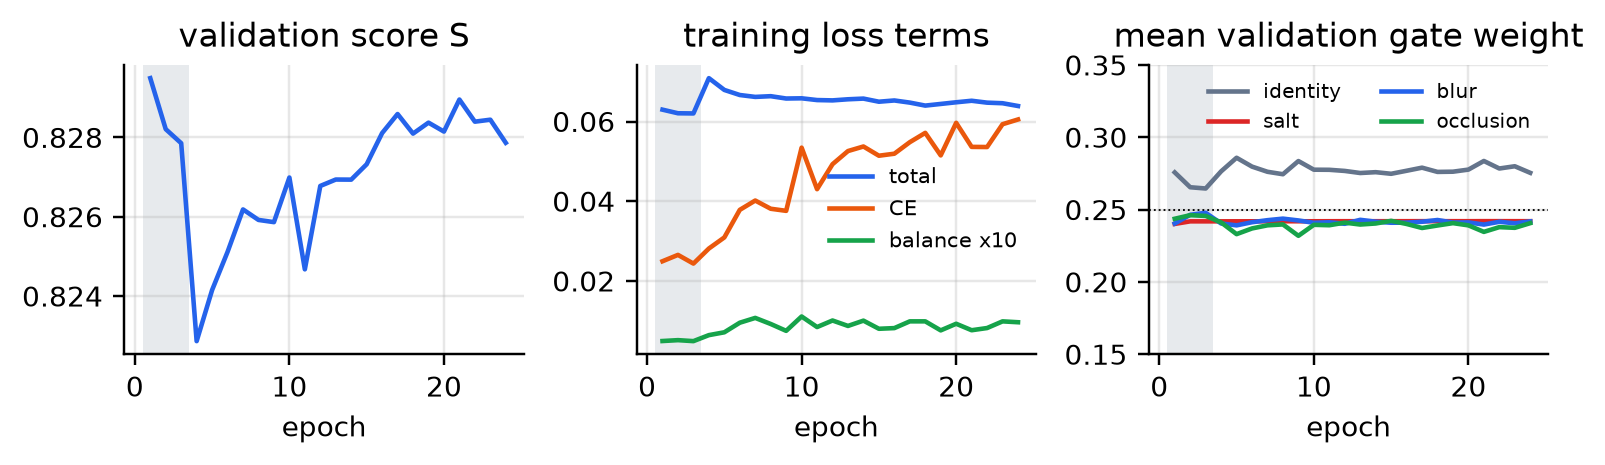
\includegraphics[width=0.55\textwidth]{t3_curves.png}\hfill
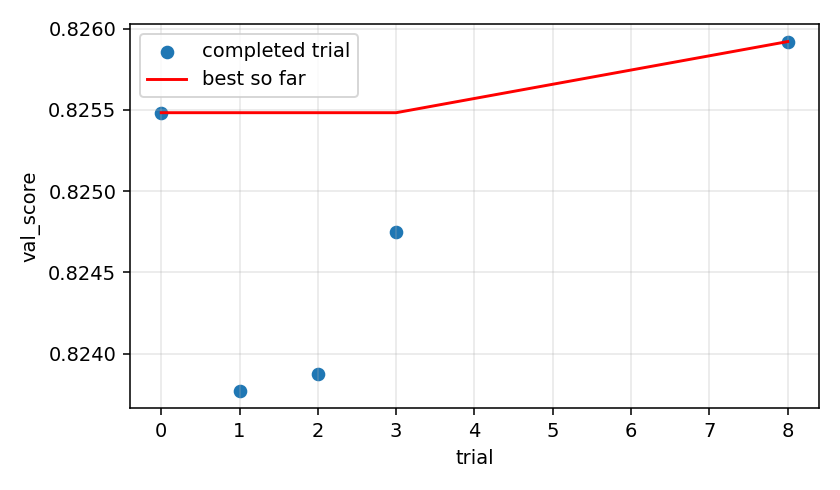
\includegraphics[width=0.235\textwidth]{t3_optuna_history.png}\hfill
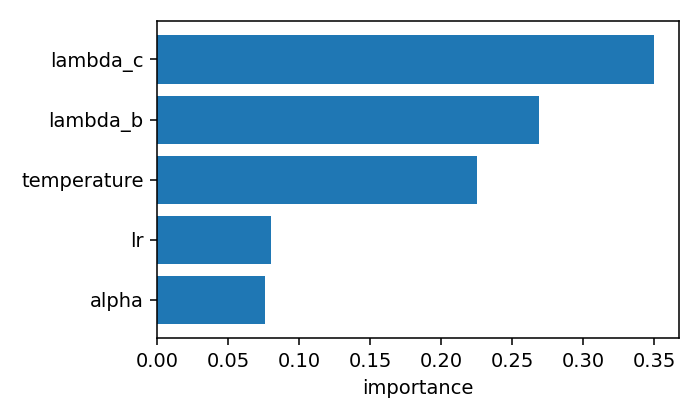
\includegraphics[width=0.19\textwidth]{t3_optuna_importance.png}
\caption{Soft-MoE training (shaded: gate warm-up with frozen experts): validation score, training loss terms, mean validation gate weight per branch (dotted: 0.25), and the Optuna history and importances.}
\label{fig:t3curves}
\end{figure*}

\subsection{Reconstruction results}
Table~\ref{tab:t3type} compares the three systems on the official test set and Table~\ref{tab:sev3} by severity; the validation set gives the same ranking. The soft MoE is within 0.13\,dB of hard routing on salt-and-pepper and blur and slightly worse on clean images, because a few percent of weight leaks to the experts. Occlusion is the interesting case: the soft model has the \emph{best} SSIM (0.760) but a 0.5\,dB lower PSNR than hard routing. The difference comes entirely from low-severity occlusion (22.5 vs.\ 24.0\,dB, but SSIM 0.863 vs.\ 0.784), where the gate splits its weight between identity and the occlusion expert (Section~\ref{sec:gate}). The blended output keeps the sharp unoccluded content from the identity branch, which SSIM rewards, but also a semi-transparent ``ghost'' of the black box, which PSNR penalises.

\begin{table}[t]
\caption{Soft MoE vs.\ hard routing (predicted) vs.\ universal model, official test set (PSNR dB / SSIM).}
\label{tab:t3type}
\centering\footnotesize
\setlength{\tabcolsep}{3.5pt}
\begin{tabular}{@{}lrrrrrr@{}}
\toprule
 & \multicolumn{2}{c}{Soft MoE} & \multicolumn{2}{c}{Hard (pred.)} & \multicolumn{2}{c}{Universal}\\
\cmidrule(lr){2-3}\cmidrule(lr){4-5}\cmidrule(l){6-7}
Type & PSNR & SSIM & PSNR & SSIM & PSNR & SSIM\\
\midrule
Salt-and-pepper & 26.96 & 0.839 & 27.07 & 0.842 & 26.61 & 0.818\\
Blur & 26.68 & 0.818 & 26.62 & 0.814 & 26.37 & 0.798\\
Occlusion & 21.68 & 0.760 & 22.22 & 0.730 & 22.08 & 0.724\\
Clean & 49.58 & 0.999 & 49.86 & 0.999 & 26.89 & 0.831\\
\midrule
Corrupted-only mean & 25.10 & 0.806 & 25.30 & 0.795 & 25.02 & 0.780\\
\bottomrule
\end{tabular}
\end{table}

\begin{table}[t]
\caption{Test-set PSNR (dB) of the three restoration systems by corruption type and severity (SSIM in parentheses for occlusion).}
\label{tab:sev3}
\centering\footnotesize
\setlength{\tabcolsep}{4pt}
\begin{tabular}{@{}llrrrr@{}}
\toprule
Type & Sev. & Input & Universal & Hard & Soft\\
\midrule
\multirow{3}{*}{Salt-pepper} & low & 20.14 & 26.84 & 27.21 & 27.08\\
 & med & 15.88 & 26.68 & 27.11 & 27.01\\
 & high & 13.14 & 26.31 & 26.90 & 26.77\\
\midrule
\multirow{3}{*}{Blur} & low & 32.27 & 27.03 & 27.00 & 27.29\\
 & med & 26.74 & 26.82 & 27.09 & 27.02\\
 & high & 24.33 & 25.27 & 25.75 & 25.73\\
\midrule
\multirow{3}{*}{Occlusion} & low & 16.69 & 23.97 (.78) & 24.00 (.78) & 22.49 (.86)\\
 & med & 13.27 & 22.16 (.73) & 22.32 (.74) & 22.28 (.75)\\
 & high & 10.76 & 20.10 (.66) & 20.35 (.67) & 20.27 (.66)\\
\bottomrule
\end{tabular}
\end{table}

\subsection{Gating analysis}\label{sec:gate}
Table~\ref{tab:gate} gives the mean test-set weights for every true corruption type and severity, and Fig.~\ref{fig:t3vis} shows them as a heat-map together with examples. The gate is almost one-hot: 86.3\% of all test samples give more than 90\% of the weight to a single branch and only 2.3\% have no branch above 60\%. The branch with the largest weight is correct for 99.9\% (blur), 99.7\% (clean), 85.4\% (occlusion) and 100\% (salt-and-pepper) of the images. No expert is inactive (mean weights: identity 0.157, salt 0.300, blur 0.291, occlusion 0.251; the identity share is lower only because clean images are 10\% of the test set) and none dominates unrelated inputs (mean weight on other classes: identity 0.068, experts $\le$0.006).

\begin{table}[t]
\caption{Mean gate weights per true corruption and severity (official test set).}
\label{tab:gate}
\centering\footnotesize
\begin{tabular}{@{}llrrrr@{}}
\toprule
True type & Sev. & Identity & Salt exp. & Blur exp. & Occl. exp.\\
\midrule
Clean & -- & \textbf{0.958} & 0.000 & 0.011 & 0.031\\
\midrule
\multirow{3}{*}{Salt-pepper} & low & 0.000 & \textbf{0.999} & 0.000 & 0.001\\
 & med & 0.000 & \textbf{1.000} & 0.000 & 0.000\\
 & high & 0.000 & \textbf{1.000} & 0.000 & 0.000\\
\midrule
\multirow{3}{*}{Blur} & low & 0.068 & 0.000 & \textbf{0.926} & 0.005\\
 & med & 0.012 & 0.000 & \textbf{0.987} & 0.001\\
 & high & 0.011 & 0.000 & \textbf{0.987} & 0.001\\
\midrule
\multirow{3}{*}{Occlusion} & low & 0.438 & 0.001 & 0.001 & \textbf{0.560}\\
 & med & 0.078 & 0.001 & 0.000 & \textbf{0.922}\\
 & high & 0.006 & 0.000 & 0.000 & \textbf{0.994}\\
\bottomrule
\end{tabular}
\end{table}

Distributed weights occur almost only for low-severity occlusion (identity 0.44, occlusion expert 0.56 on average), the same pair that the classifier confuses. For 74\% of these images the identity weight exceeds 0.2, and those inputs have a higher input PSNR (17.1 vs.\ 15.5\,dB), i.e.\ the single box falls on darker, less informative regions. The lower rows of Fig.~\ref{fig:t3vis} show exactly this: dark cats or dark backgrounds with a small box, weights split roughly evenly, and a soft output in which the box is only partly removed. Mild blur shows a much weaker version of the same effect (6.8\% identity weight).

\begin{figure*}[t]
\centering
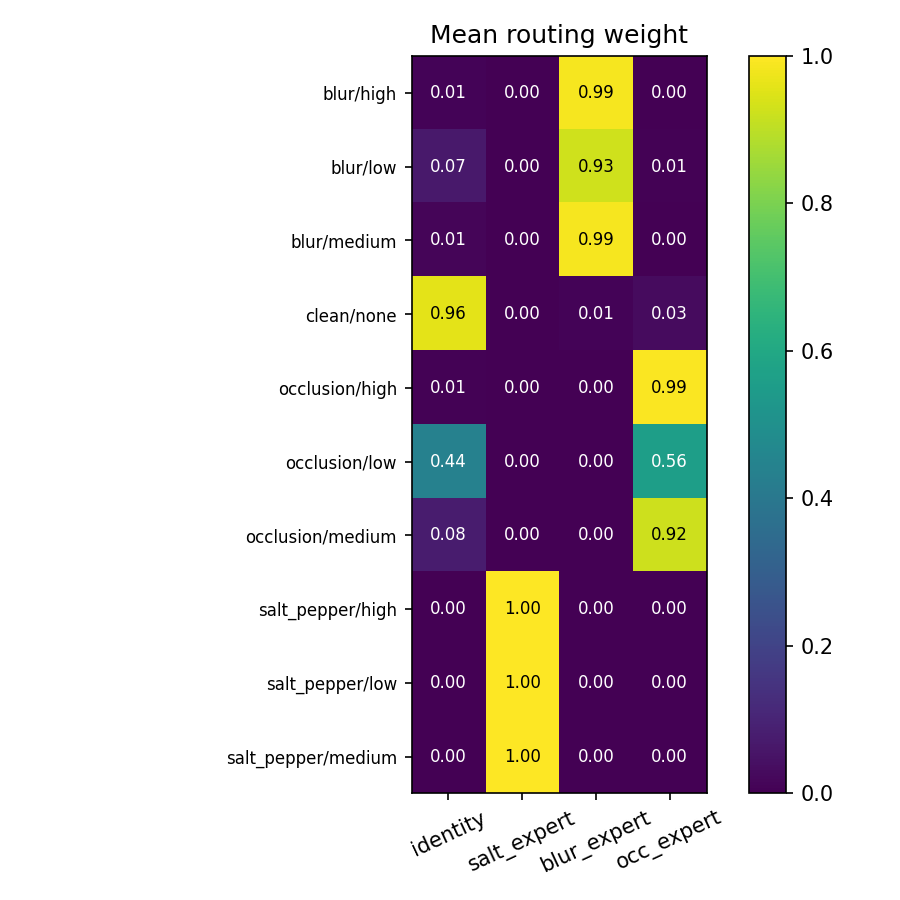
\includegraphics[height=0.3\textheight]{t3_heatmap_test.png}\hspace{8mm}
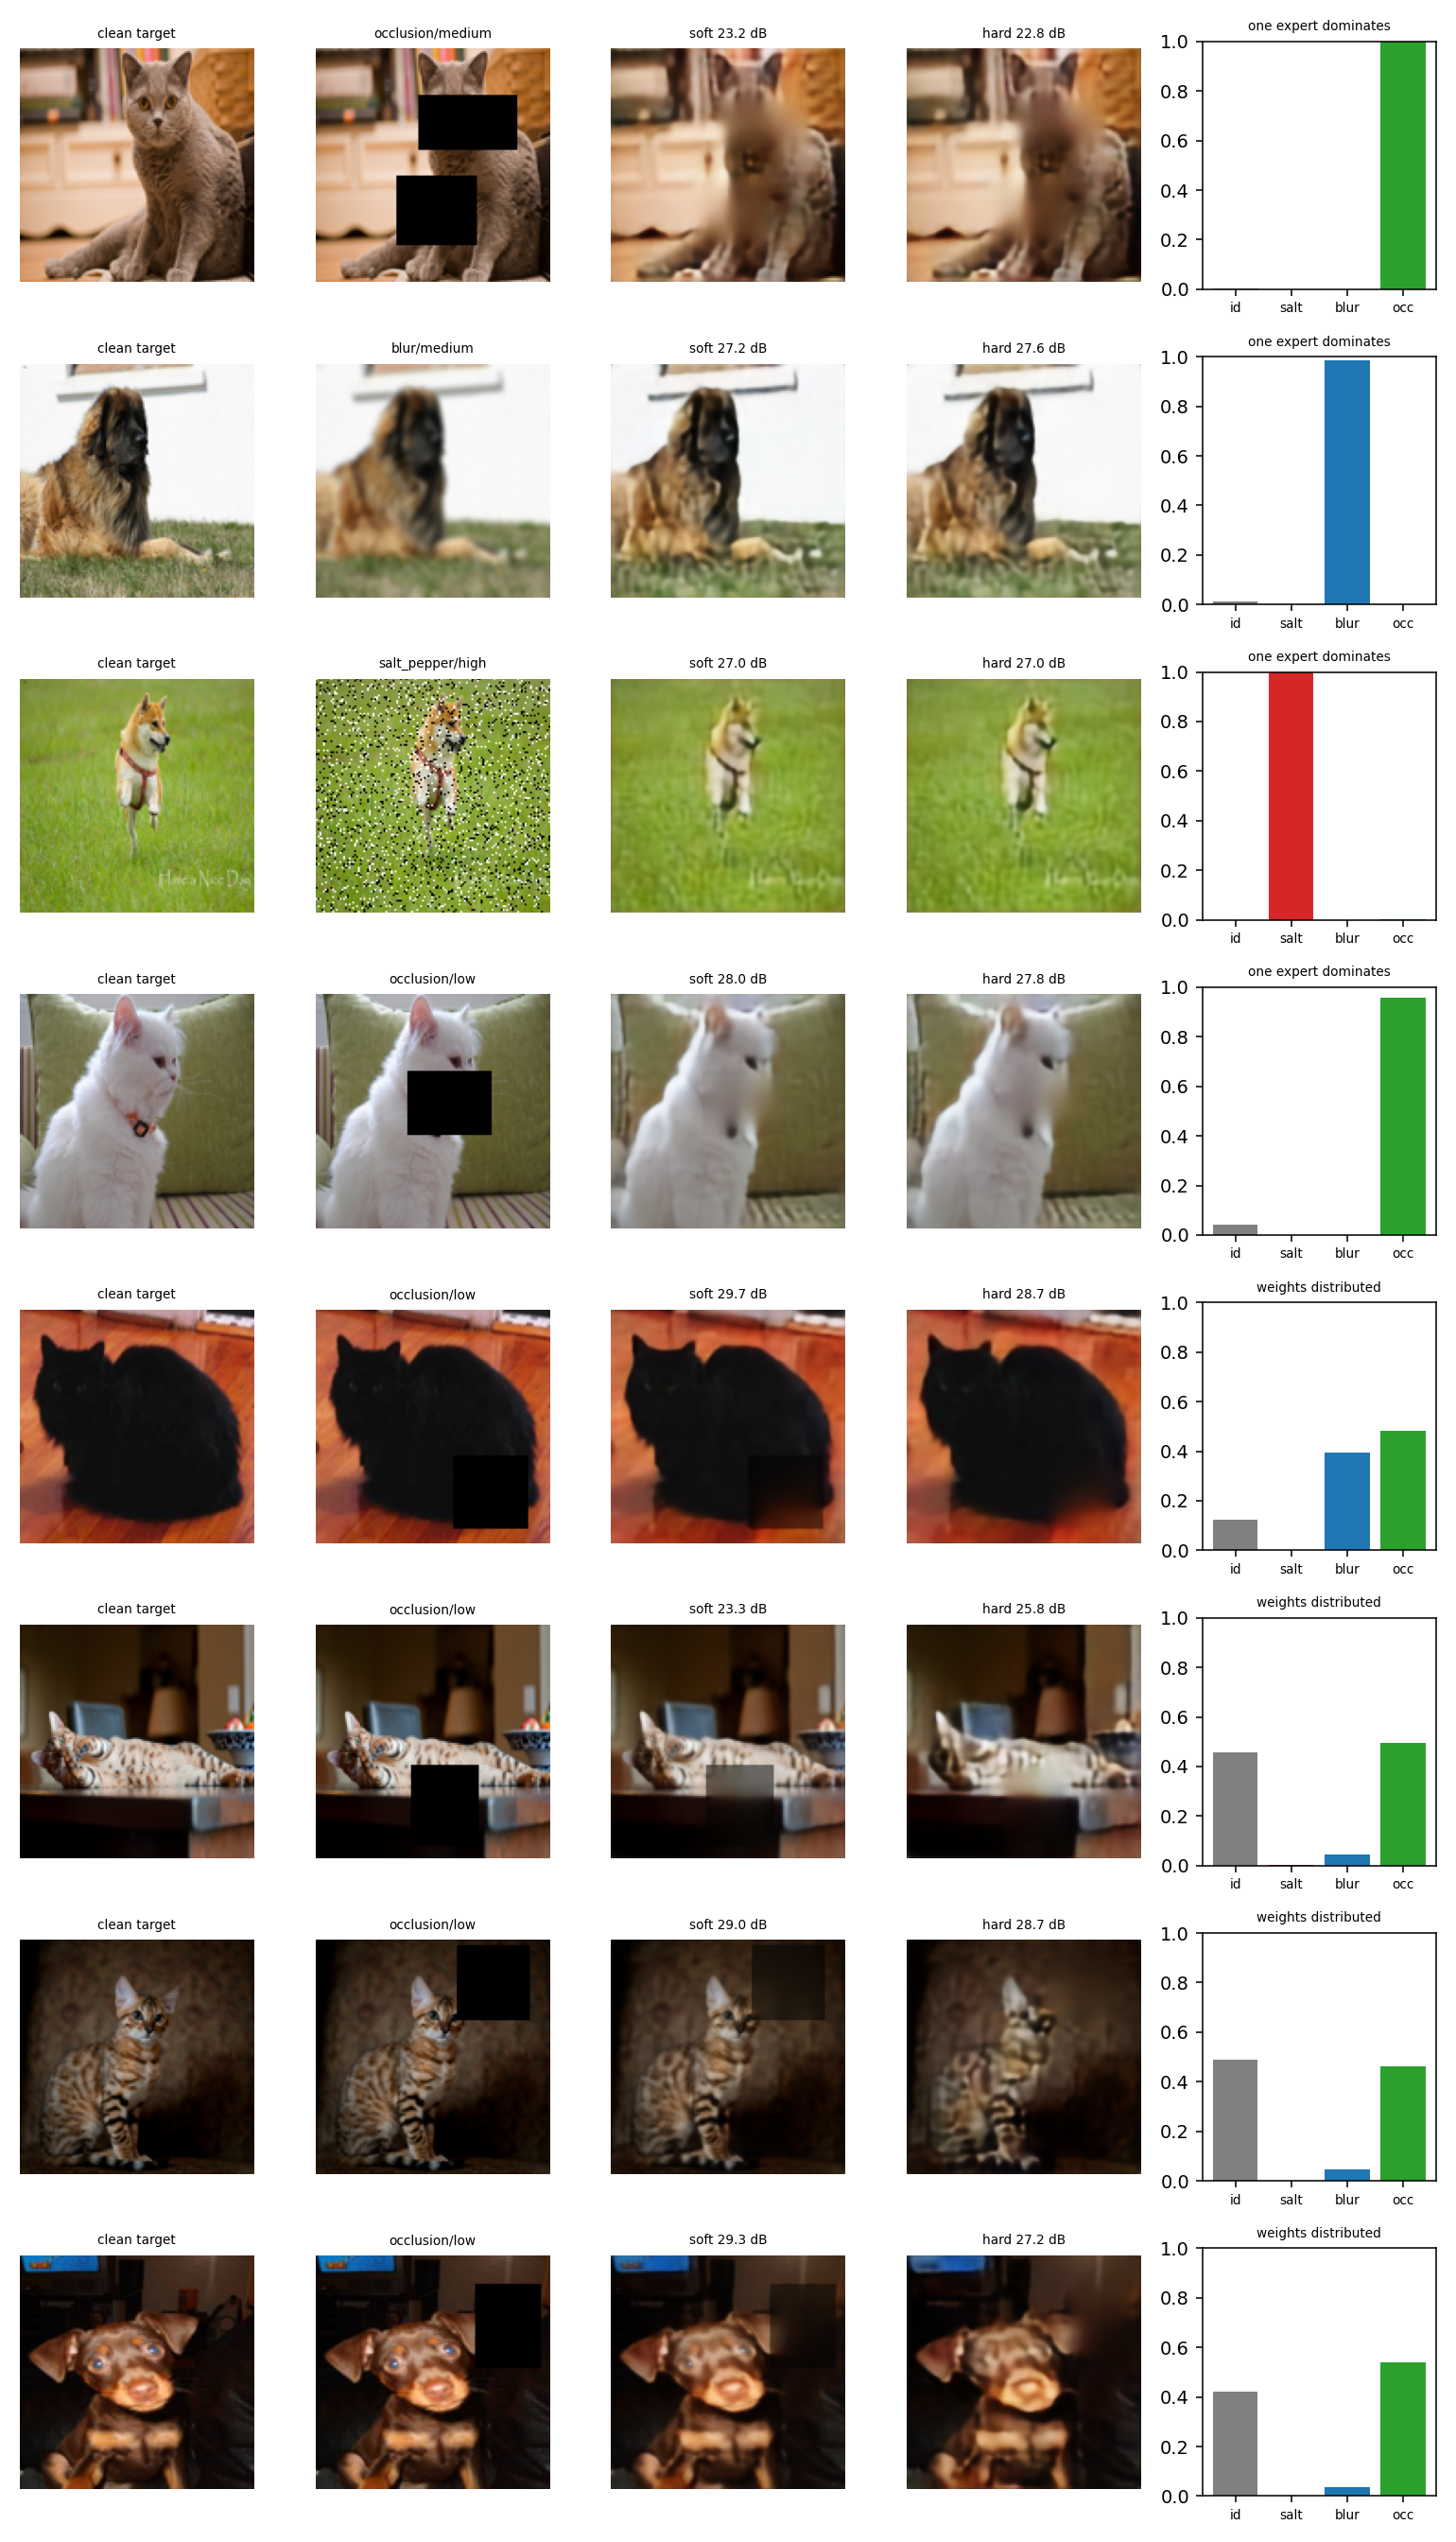
\includegraphics[height=0.5\textheight]{t3_gate_examples_test.png}
\caption{Gating behaviour on the official test set. Left: mean routing weight per true corruption and severity. Right: examples in which one expert dominates (top four rows) and in which the weights are distributed (bottom four rows, all low-severity occlusions), with soft- and hard-routing outputs and PSNR.}
\label{fig:t3vis}
\end{figure*}

\subsection{Mixed corruptions: a negative result}
Soft routing is motivated by images with more than one corruption. We applied blur+noise, noise+occlusion and blur+occlusion to test images (Table~\ref{tab:mixed}; the validation run with 300 images per mix gives the same picture). On every combination the gate put $\ge$99.7\% of its weight on a single expert, so soft routing behaved like hard routing, and the \emph{universal model was best}. For noise+occlusion the gate chose the noise expert and left the boxes unrepaired (13.8\,dB against 21.6\,dB for the universal model).

\begin{table}[t]
\caption{Mixed-corruption stress test, official test images (PSNR dB / SSIM).}
\label{tab:mixed}
\centering\footnotesize
\setlength{\tabcolsep}{3pt}
\begin{tabular}{@{}lrrrr@{}}
\toprule
Mix & Input & Soft MoE & Hard & Universal\\
\midrule
Blur + salt-pepper & 15.45/0.24 & 25.42/0.77 & 25.42/0.77 & \textbf{25.89/0.78}\\
Salt-pepper + occl. & 11.86/0.25 & 13.79/0.62 & 13.63/0.61 & \textbf{21.63/0.72}\\
Blur + occlusion & 13.58/0.58 & 21.93/0.68 & 21.95/0.68 & \textbf{22.20/0.72}\\
\bottomrule
\end{tabular}
\end{table}

The reason is structural: the output is a convex combination of expert \emph{outputs}. For two simultaneous degradations each expert repairs only one, so any blend retains the other. Composing experts requires a cascade or a feature-level mixture, and the universal model, trained on all single corruptions, generalises to combinations. A proposed remedy (training with compound corruptions and a higher temperature) was not attempted for lack of time.

\subsection{Cost and export}
The full pipeline (gate, three experts, identity, weighted sum) is exported as one ONNX file of 84.5\,MB with outputs \texttt{restored} and \texttt{weights}; the maximum difference to PyTorch is $1.3\times10^{-6}$. Because the soft model always runs all three experts, one image takes 133\,ms on a CPU against about 47\,ms for hard routing (Table~\ref{tab:onnx}); a roughly three-fold cost buys a small SSIM gain on occlusion but no PSNR gain on the data tested.

% =====================================================================
\section{Task 4: Style-Conditioned Face-to-Sketch cGAN}
\subsection{Architecture}
\textbf{Generator.} A U-Net with seven stride-2 encoder blocks ($128\to1$), six decoder blocks with skip connections and an output layer, tanh output (Fig.~\ref{fig:t4arch}). The style $s\in\{0,1,2\}$ is a learned embedding that enters in two places: it is tiled spatially and concatenated to the photo at the input, and it drives a FiLM modulation (scale and shift predicted from the embedding, initialised to the identity) after the normalisation of every decoder block. Dropout is applied in the first three decoder blocks. \textbf{Discriminator.} A conditional PatchGAN receives the photo, the real or generated sketch and the tiled embedding of its own embedding table and outputs a $14{\times}14$ map of patch logits.

\begin{figure*}[t]
\centering
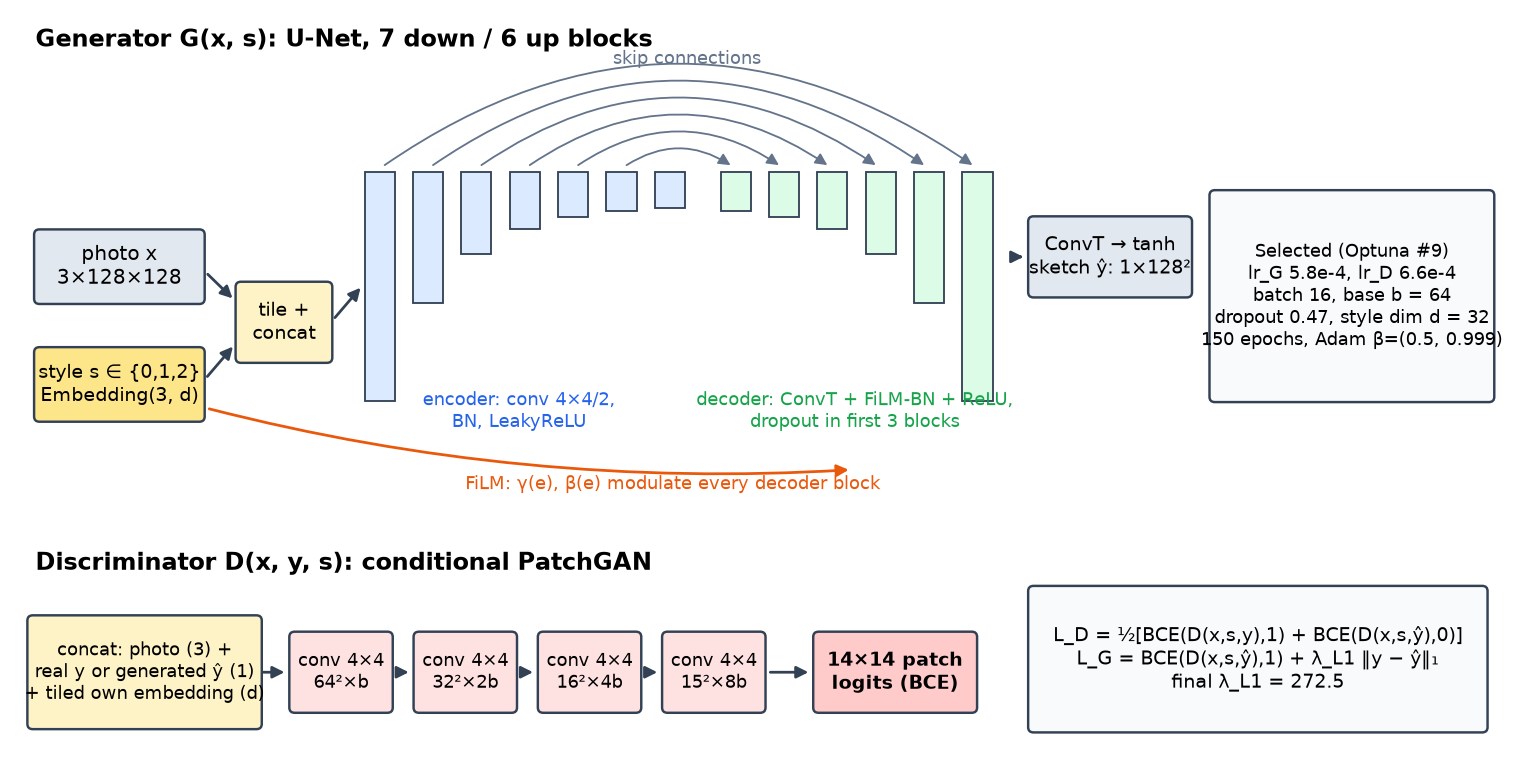
\includegraphics[width=0.86\textwidth]{t4_arch.png}
\caption{Task 4 networks. Top: U-Net generator; the style embedding is concatenated to the photo and modulates every decoder block through FiLM. Bottom: conditional PatchGAN discriminator with its own style embedding, and the losses.}
\label{fig:t4arch}
\end{figure*}

\subsection{Losses and training}
With photo $x$, style $s$, real sketch $y$ and $\hat y=G(x,s)$, the discriminator minimises a binary cross-entropy with logits,
\begin{equation}
\mathcal{L}_D=\tfrac12\bigl[\mathrm{BCE}(D(x,s,y),1)+\mathrm{BCE}(D(x,s,\hat y),0)\bigr],
\end{equation}
and the generator
\begin{equation}
\mathcal{L}_G=\mathrm{BCE}(D(x,s,\hat y),1)+\lambda_{L1}\lVert y-\hat y\rVert_1.
\end{equation}
The four components (D-real, D-fake, G-adversarial, G-$\ell_1$) are logged separately, with validation $\ell_1$, SSIM and PSNR (Figs.~\ref{fig:mlflow} and~\ref{fig:t4curves}), and the same eight validation photos are rendered in all three styles every five epochs (Fig.~\ref{fig:t4samples}). Spatial augmentation (horizontal flip, random crop of 80--100\% and resize) is applied to the \emph{stacked} photo+sketch tensor, so both always receive the identical transform. The Optuna study (20 trials of 20 epochs; Tables~\ref{tab:search}--\ref{tab:optuna}) preferred a large $\lambda_{L1}=272.5$ (the suggested value is 100) with high dropout 0.47; the learning rates and dropout dominate (Table~\ref{tab:importance}). The selected configuration was retrained for 150 epochs ($\approx$11\,s per epoch). The adversarial losses settle after about 20 epochs; apart from one transient spike near epoch 65, the discriminator losses then stay balanced (last 30 epochs: real $\approx$0.45, fake $\approx$0.39) and the generator adversarial loss is steady ($\approx$1.9), i.e.\ neither network collapsed, while the training $\ell_1$ keeps decreasing. Validation SSIM fluctuates between 0.49 and 0.51.

\begin{figure*}[t]
\centering
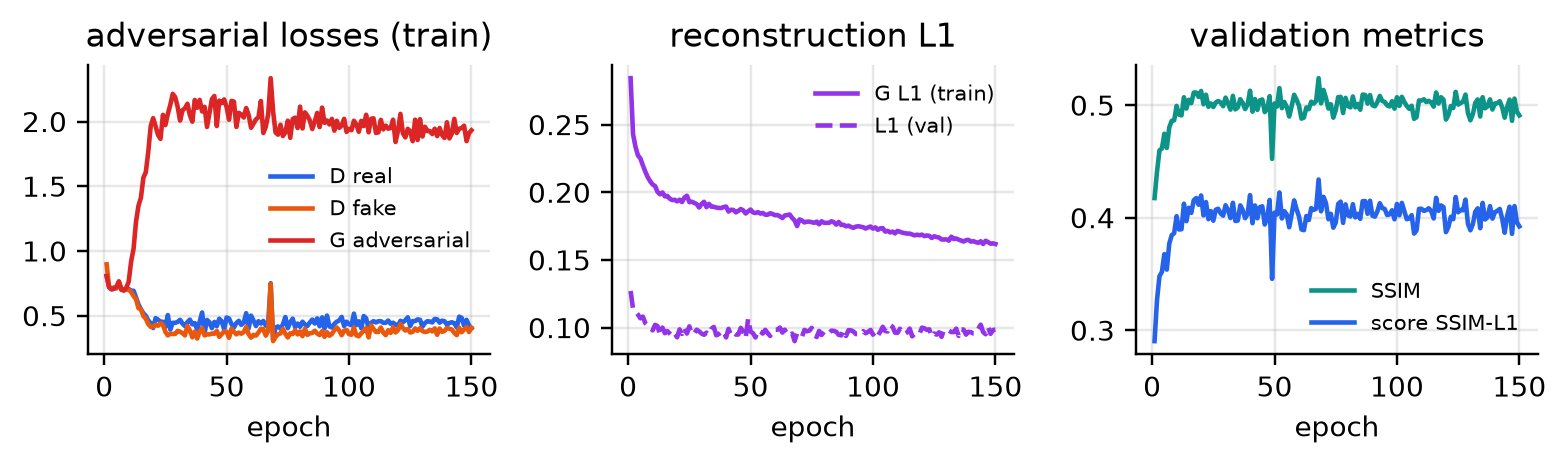
\includegraphics[width=0.6\textwidth]{t4_curves.png}\hfill
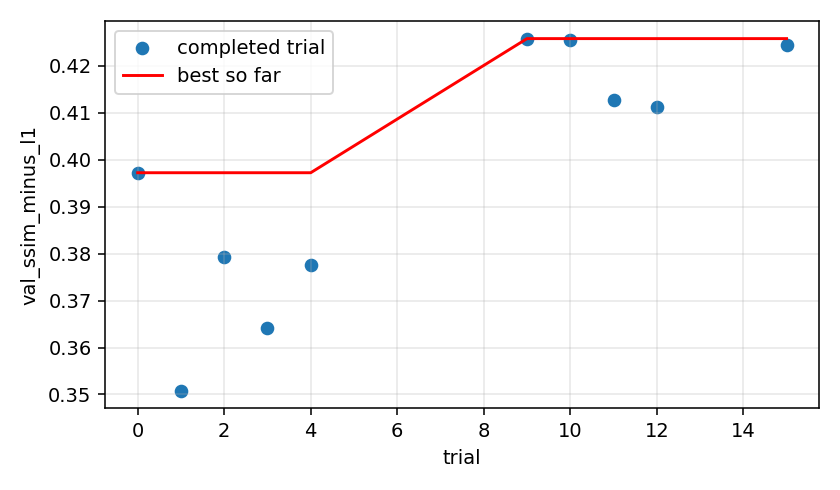
\includegraphics[width=0.21\textwidth]{t4_optuna_history.png}\hfill
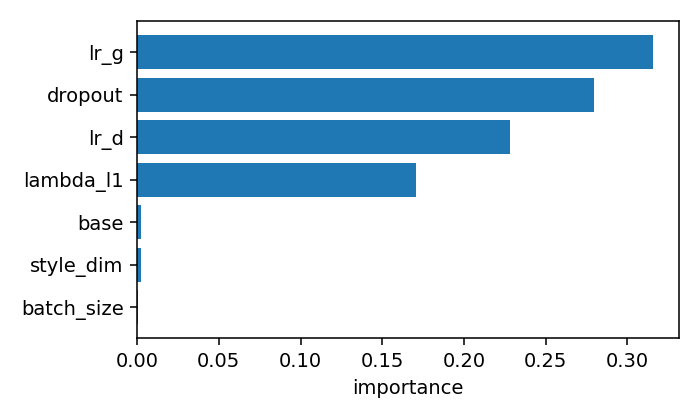
\includegraphics[width=0.17\textwidth]{t4_optuna_importance.png}
\caption{cGAN training: the four separately logged loss components, training and validation $\ell_1$, validation SSIM and score, and the Optuna history and importances.}
\label{fig:t4curves}
\end{figure*}

\begin{figure*}[t]
\centering
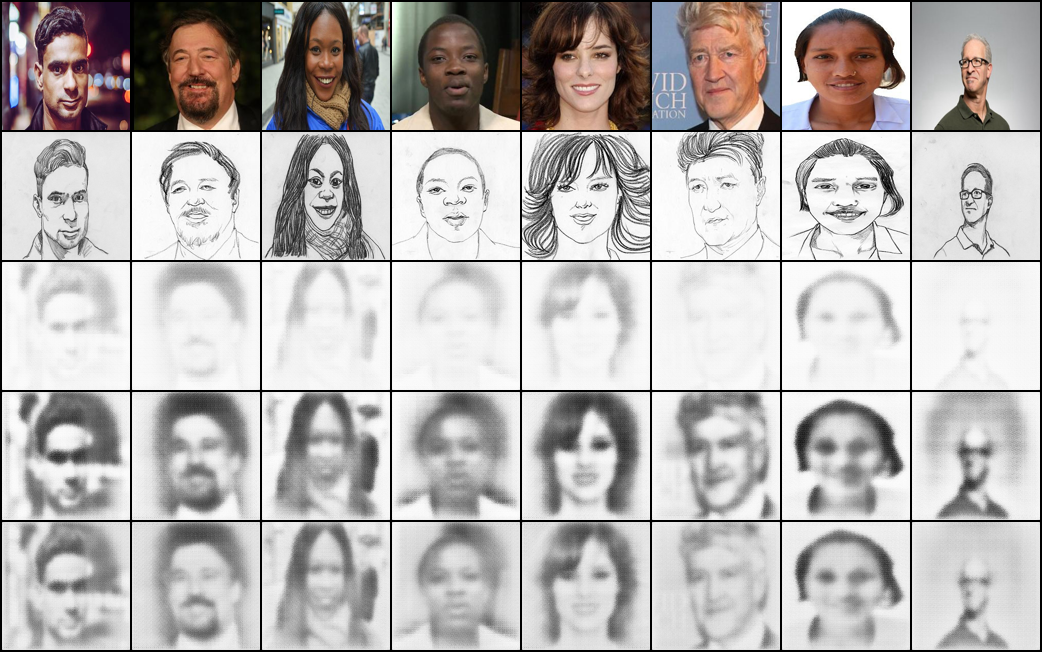
\includegraphics[width=0.325\textwidth]{t4_samples_ep000.png}\hfill
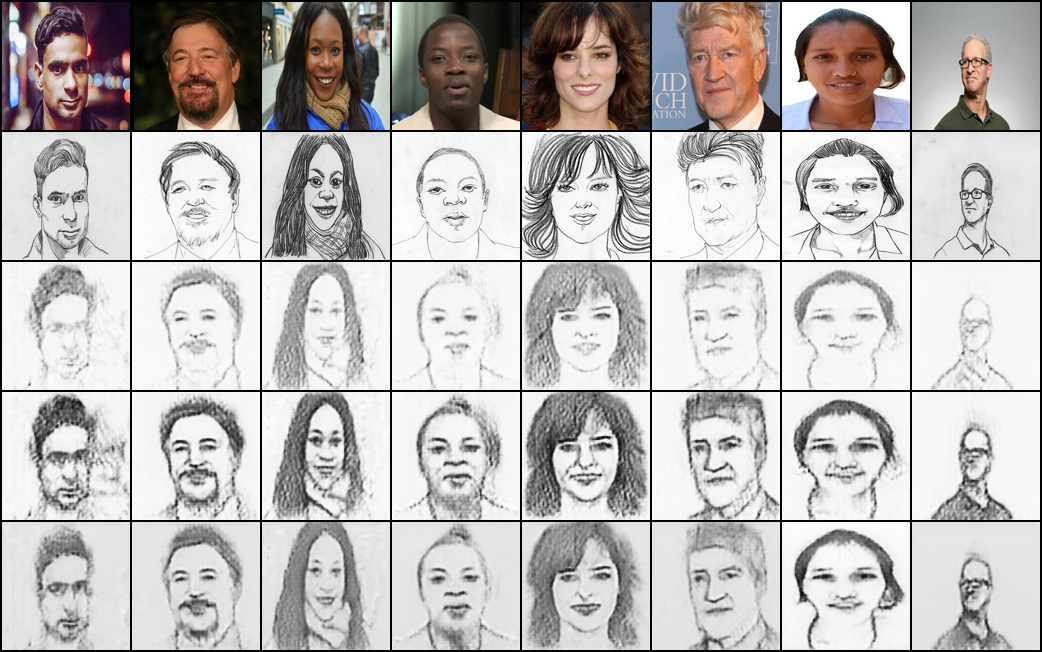
\includegraphics[width=0.325\textwidth]{t4_samples_ep050.png}\hfill
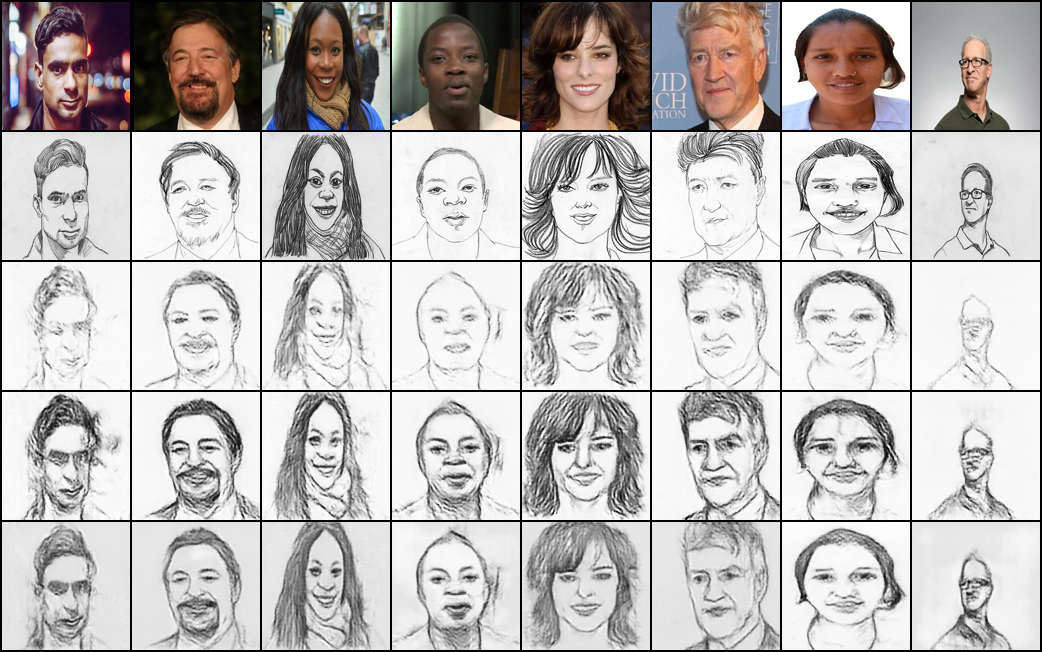
\includegraphics[width=0.325\textwidth]{t4_samples_ep149.png}
\caption{The same fixed validation photos after epochs 0, 50 and 149 (rows: photo, ground truth, generated in style 0, 1, 2). Early outputs are grey blobs; by epoch 50 the facial layout and hair contours appear; later epochs mainly sharpen the strokes.}
\label{fig:t4samples}
\end{figure*}

\subsection{Results}
The model clearly beats the trivial baseline (Table~\ref{tab:t4}: SSIM 0.524 against 0.288; $\ell_1$ 0.090 against 0.405). Style 1 is the hardest ($\ell_1$ 0.125). \textbf{Is the condition used?} Table~\ref{tab:swap} generates every validation photo in all three styles and compares with the ground truth. For every true style the best SSIM and lowest $\ell_1$ lie on the diagonal, and outputs for different styles of the same photo differ by 0.09--0.12 in mean absolute pixel difference, so the embedding changes the output in the intended way and is not just an interface label. Because training styles are correlated with the photo source (Section~III-B), part of this effect could be driven by the photo; the off-diagonal degradation shows the label itself matters.

\begin{table}[t]
\caption{Task 4, validation set, generated with the true style ($\ell_1$ and PSNR on the [0,1] scale). Baseline: the grayscale photo used as the sketch.}
\label{tab:t4}
\centering\footnotesize
\begin{tabular}{@{}lrrrrr@{}}
\toprule
Style & $n$ & $\ell_1$ & SSIM & PSNR & Base SSIM\\
\midrule
0 & 54 & 0.070 & 0.534 & 18.41 & 0.260\\
1 & 52 & 0.125 & 0.436 & 13.99 & 0.239\\
2 & 53 & 0.077 & 0.600 & 17.75 & 0.364\\
All & 159 & 0.090 & 0.524 & 16.75 & 0.288\\
\bottomrule
\end{tabular}
\end{table}

\begin{table}[t]
\caption{Style-conditioning check, validation. Rows: true style; columns: style the generator was told. Mean SSIM (left) and mean $\ell_1$ (right).}
\label{tab:swap}
\centering\footnotesize
\begin{tabular}{@{}lrrrrrr@{}}
\toprule
 & \multicolumn{3}{c}{SSIM} & \multicolumn{3}{c}{$\ell_1$}\\
\cmidrule(lr){2-4}\cmidrule(l){5-7}
True & c0 & c1 & c2 & c0 & c1 & c2\\
\midrule
0 & \textbf{0.534} & 0.439 & 0.491 & \textbf{0.070} & 0.137 & 0.118\\
1 & 0.395 & \textbf{0.436} & 0.418 & 0.143 & \textbf{0.125} & 0.141\\
2 & 0.522 & 0.489 & \textbf{0.600} & 0.128 & 0.128 & \textbf{0.077}\\
\bottomrule
\end{tabular}
\end{table}

\textbf{Visual results and failure cases.} Fig.~\ref{fig:t4vis} shows the three styles side by side: style~0 gives thin, light contour lines, style~1 dense dark hatching, and style~2 a lighter tonal rendering, matching the ground-truth styles. The four lowest-SSIM validation cases share one cause: \emph{long, voluminous or curly hair}. In the two style-1 failures the ground truth draws the hair with many crisp, dark pen strokes; the generator gets the head shape and facial layout right but renders the hair as a blurred grey mass with smudged strokes. In the two style-0 failures (curly and layered hair) the ground truth uses a few clean outline strokes, whereas the generator produces grey tonal shading instead of lines. The $\ell_1$ term, with its large weight, averages over the many possible stroke positions and therefore produces grey ``mean strokes''; the adversarial term sharpens faces but not these large, highly variable regions.

\begin{figure*}[t]
\centering
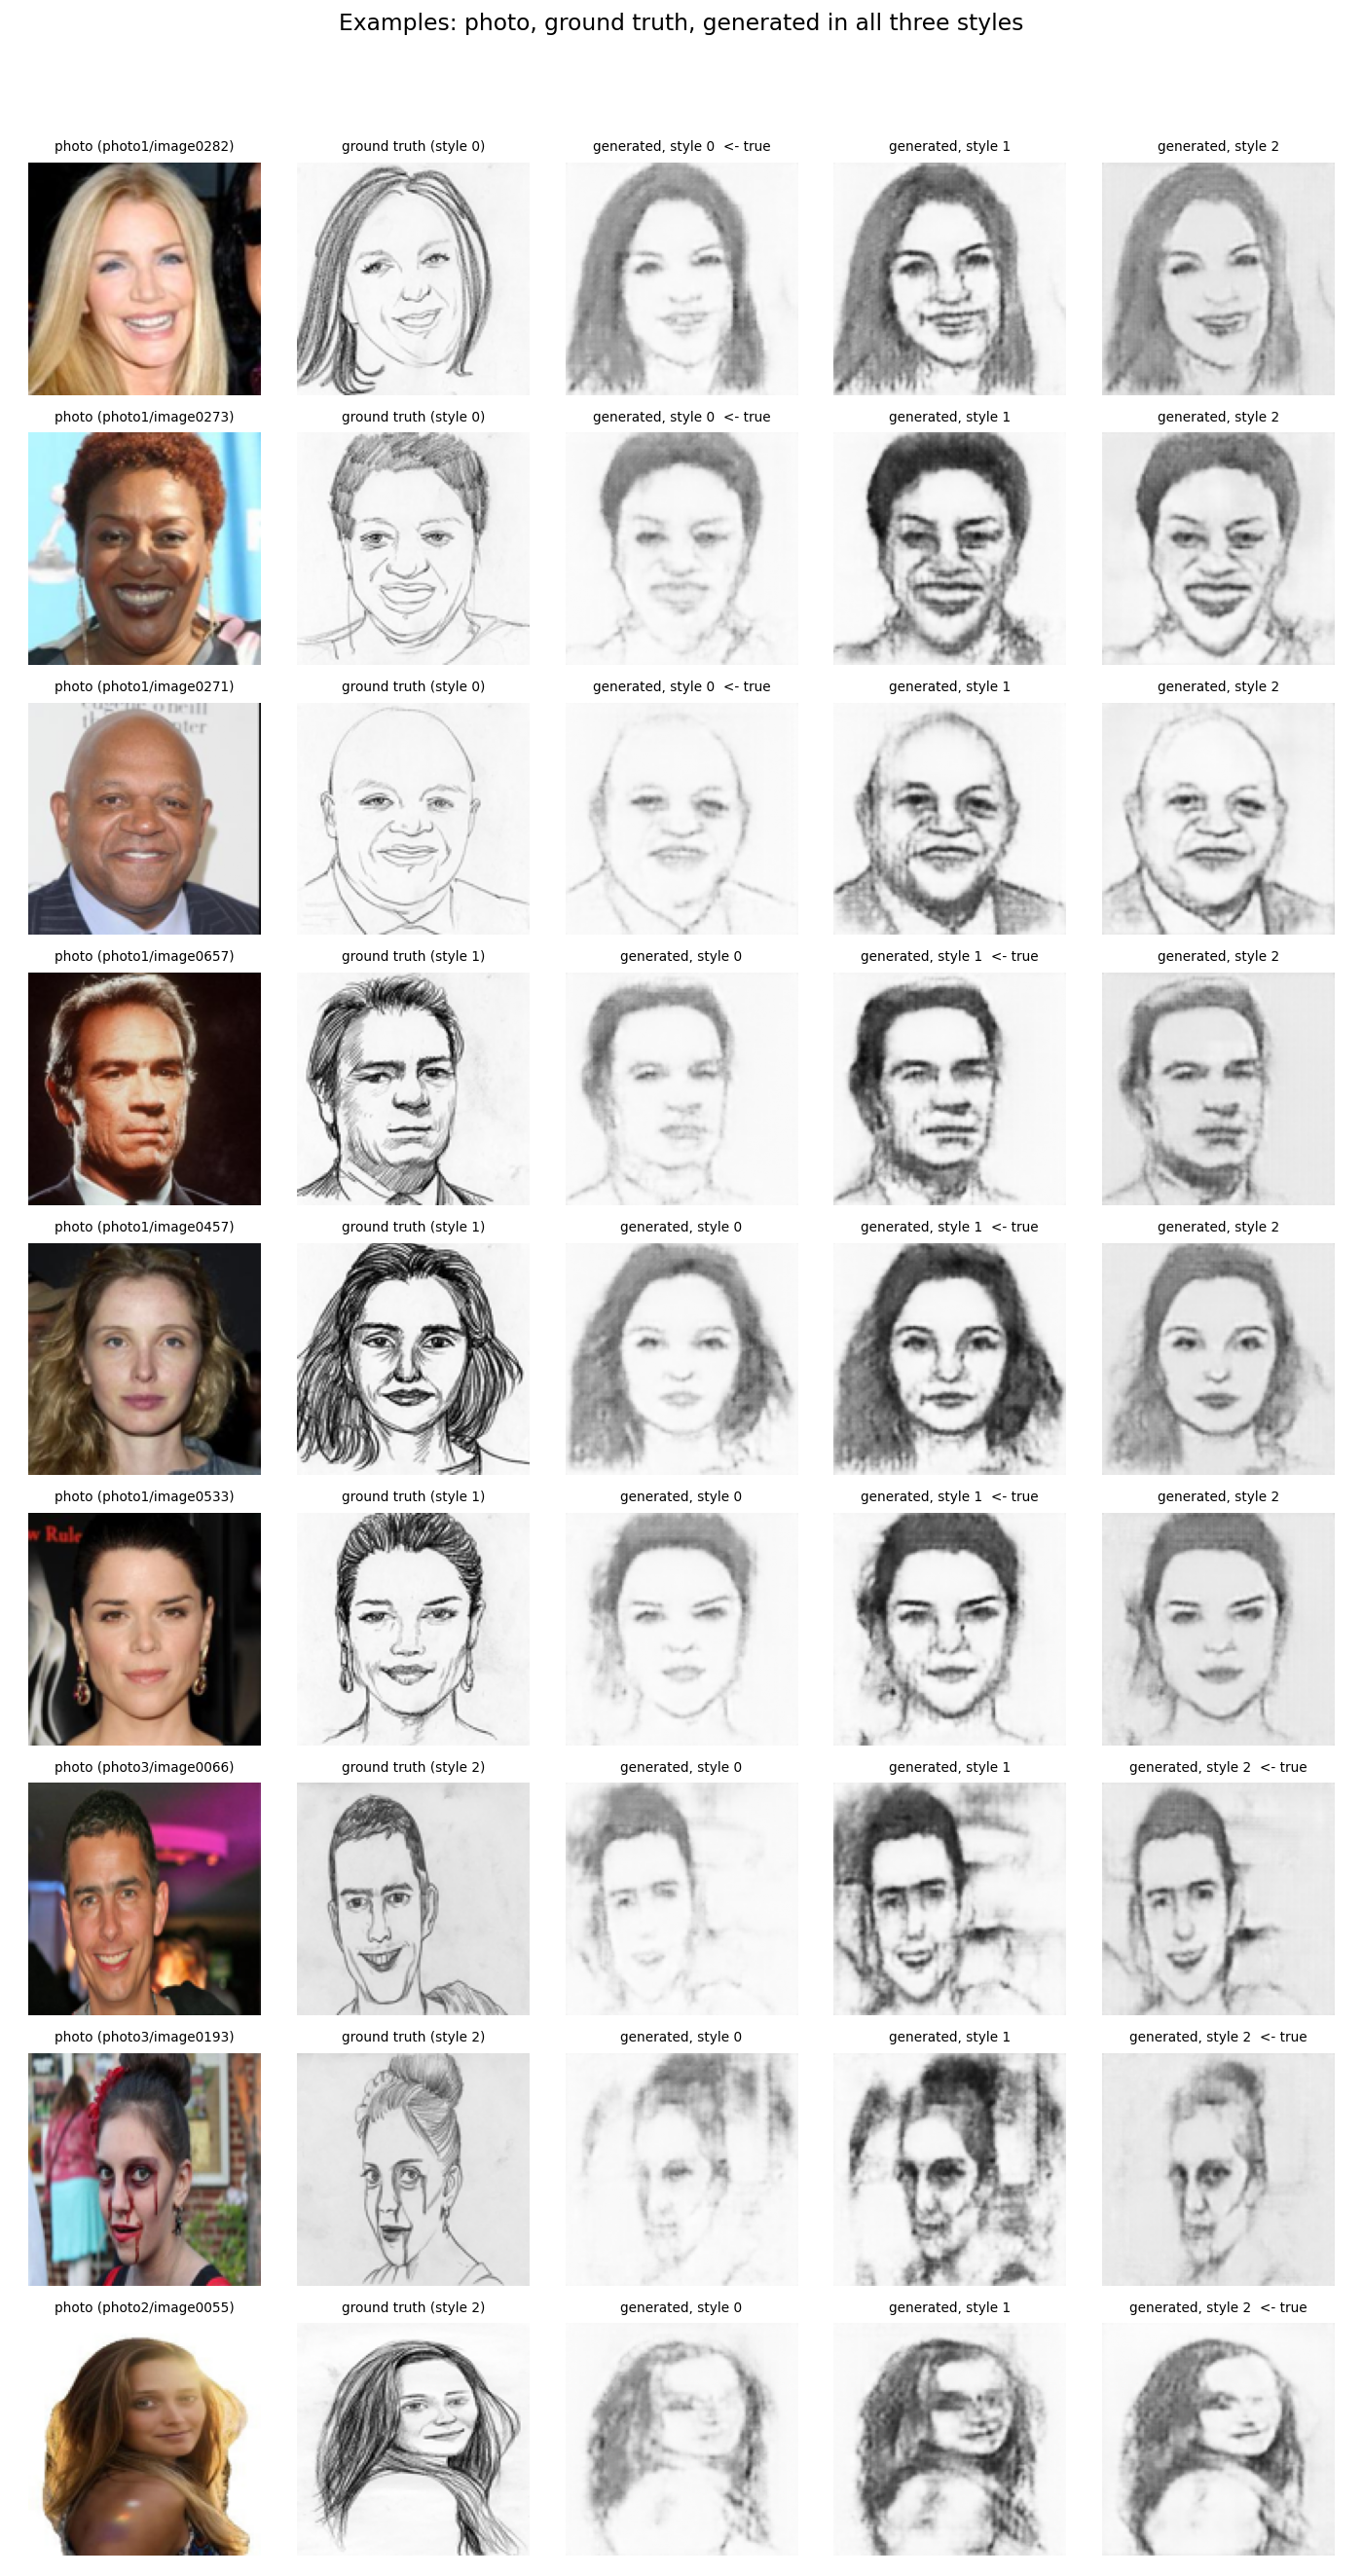
\includegraphics[height=0.42\textheight]{t4_val_examples.png}\hspace{6mm}
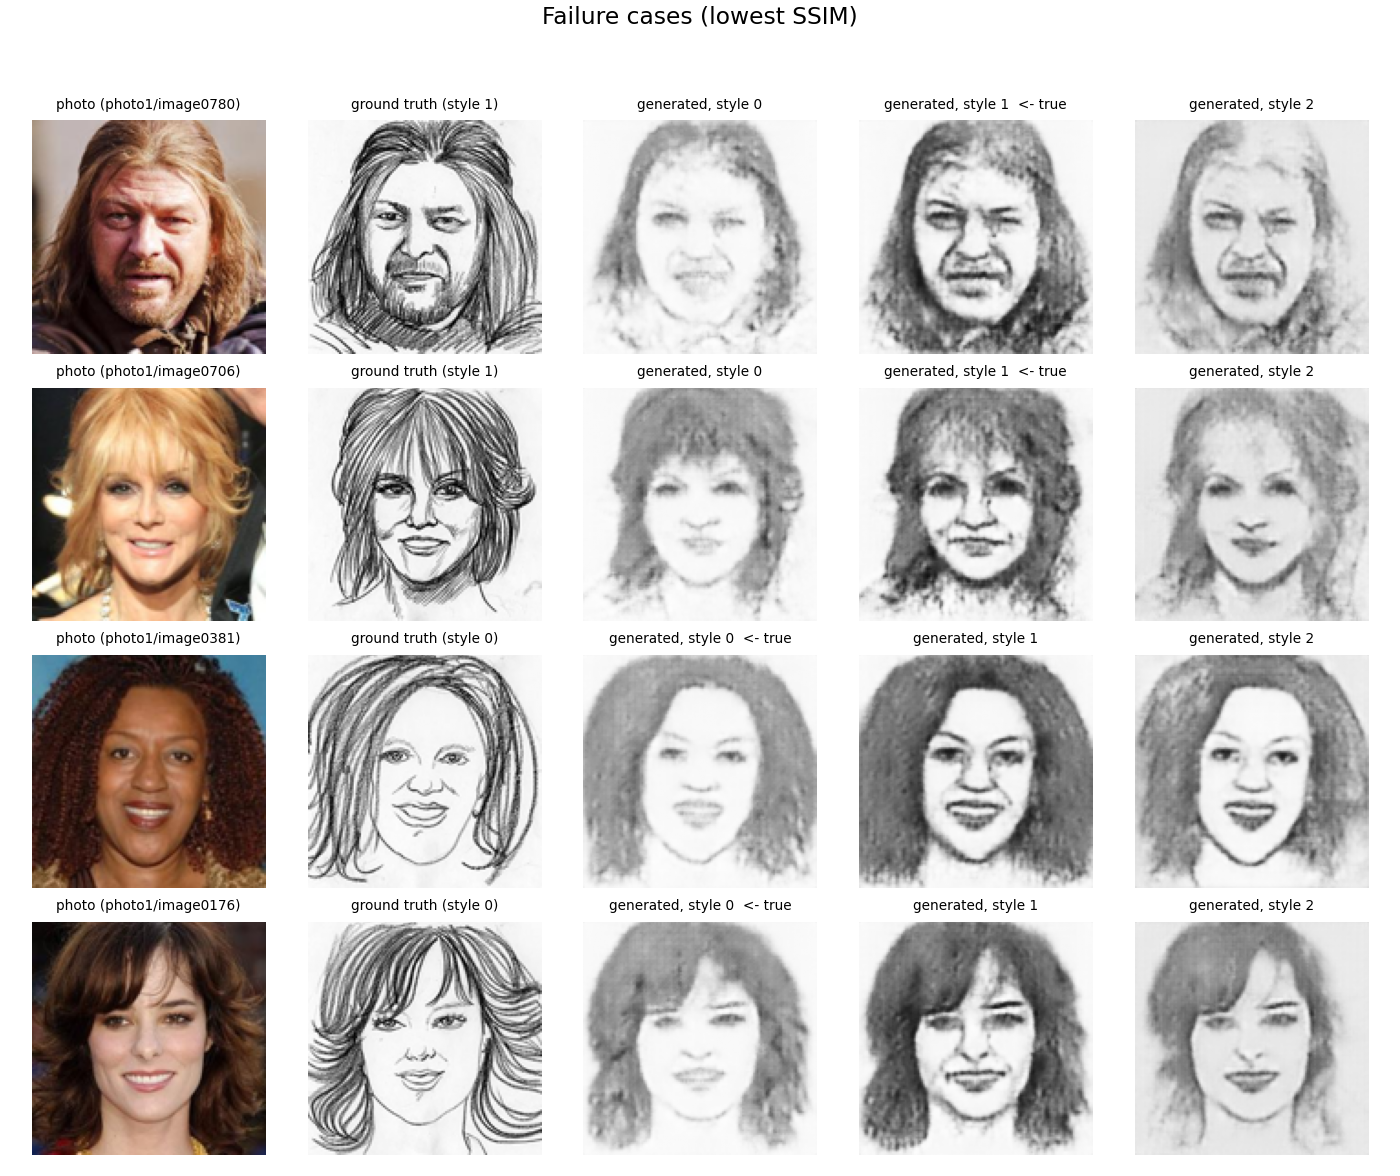
\includegraphics[height=0.25\textheight]{t4_val_failures.png}
\caption{Task 4 validation results. Left: photo, ground truth and the sketch generated in each of the three styles (the true style marked). Right: the four lowest-SSIM failure cases, all dominated by long or curly hair.}
\label{fig:t4vis}
\end{figure*}

\textbf{Caveats.} Pixel metrics only partially reflect sketch quality, so the figures matter as much as the numbers. The checkpoint was selected on the validation set, so these numbers are optimistic. The official-test evaluation of the generator was not run within the submission time, so all Task~4 numbers are validation numbers. A drop on the test set is expected from the distribution shift described in Section~III-B (59\% style~0, and 179 style-0 stock photos of a kind never seen in training).

\subsection{Export}
Only the generator is exported (168\,MB, inputs \texttt{photo} and \texttt{style}, output \texttt{sketch} in $[0,1]$; the $[-1,1]$ scaling is inside the graph). The maximum difference to PyTorch over all styles and three batch sizes is $9.8\times10^{-7}$; inference takes 29\,ms on a CPU. The file exceeds GitHub's 100\,MB limit and is therefore distributed outside the Git history.

\begin{table}[t]
\caption{ONNX export and verification (CPU, batch 1).}
\label{tab:onnx}
\centering\footnotesize
\setlength{\tabcolsep}{3pt}
\begin{tabular}{@{}lrrr@{}}
\toprule
Model & Size (MB) & Max diff & Latency (ms)\\
\midrule
T1 universal AE & 26.6 & $1.7\times10^{-6}$ & 42.1\\
T2 classifier & 4.7 & $1.2\times10^{-7}$ & 7.7\\
T2 specialist, salt-and-pepper & 26.6 & $2.6\times10^{-6}$ & 39.1\\
T2 specialist, blur & 26.6 & $1.7\times10^{-6}$ & 39.3\\
T2 specialist, occlusion & 26.6 & $2.1\times10^{-6}$ & 40.1\\
T2 routed pipeline (0 mismatches) & -- & $2.1\times10^{-6}$ & $\approx$47\\
T3 soft MoE (restored/weights) & 84.5 & $1.3/0.5\times10^{-6}$ & 132.8\\
T4 generator & 168.0 & $9.8\times10^{-7}$ & 29.3\\
\bottomrule
\end{tabular}
\end{table}

% =====================================================================
\section{Application Design and Deployment}
\subsection{Design process}
The interface was designed before implementation in Google Stitch\IfFileExists{figures/app_stitch_1.png}{ (Fig.~\ref{fig:stitch})}{}: one application with a persistent left sidebar listing the four workspaces (Universal Restoration, Hard-Routed Restoration, Soft Mixture-of-Experts Restoration, Face-to-Sketch Generator) and a system page, a light theme with rounded cards, a two-column workspace layout (input and settings on the left, results on the right), image panels at equal size so that input, output and error map can be compared directly, and a collapsing menu on small screens. The React implementation follows this structure (Fig.~\ref{fig:app}).

\IfFileExists{figures/app_stitch_1.png}{%
\begin{figure*}[t]
\centering
\includegraphics[width=0.32\textwidth]{app_stitch_1.png}\hfill
\IfFileExists{figures/app_stitch_2.png}{\includegraphics[width=0.32\textwidth]{app_stitch_2.png}}{}\hfill
\IfFileExists{figures/app_stitch_3.png}{\includegraphics[width=0.32\textwidth]{app_stitch_3.png}}{}
\caption{Original Google Stitch design of the application.}
\label{fig:stitch}
\end{figure*}}{}

\subsection{Backend}
The backend is a FastAPI service over ONNX Runtime (CPU) with the endpoints \texttt{GET /api/health}, \texttt{GET /api/samples}, \texttt{POST /api/corrupt}, \texttt{POST /api/restore/universal}, \texttt{POST /api/restore/hard}, \texttt{POST /api/restore/soft} and \texttt{POST /api/sketch}; interactive documentation is generated at \texttt{/docs}. A request carries an uploaded image (or one of the clean samples) and, for Tasks~1--3, the corruption type and severity. Uploads are validated (image content type, at most 10\,MB, decodable, PNG/JPEG/BMP/WEBP/TIFF only), converted to RGB and resized exactly as in training (bicubic, $128{\times}128$). Corruptions are produced by the same module used in training: \emph{none} (the upload is already corrupted), \emph{clean}, the three corruptions at the fixed test severities low/medium/high, a random severity from the training range, or custom parameters; the seed is returned so every run can be reproduced. The response contains the input, output, clean reference and absolute-error map as PNG images, the corruption settings (including occlusion box coordinates and the measured coverage), PSNR/SSIM of input and output whenever the clean target is known, preprocessing and inference times, and task-specific information: the four classifier probabilities, the predicted and true class, the selected expert, a routing-error flag and the separate classifier and expert times (Task~2, with predicted or oracle routing); the four routing weights, the ranking of the branches, the dominant branch and the normalised routing entropy (Task~3); and one or all three styles for Task~4. Models are loaded lazily and warmed up in a background thread at start-up; a missing model file only disables its workspace (HTTP 503), and the health endpoint reports, per model, whether it is present and loaded, its input/output signature and its ONNX-versus-PyTorch export report. The API was first tested with dummy ONNX models that have the same input/output signatures as the real ones (routing for each class including the identity bypass, oracle mode without a known label, all styles, invalid uploads and parameters) and then end-to-end with the trained models inside the Docker deployment.

\subsection{Frontend}
The frontend is written in React with Tailwind CSS and built with Vite (Fig.~\ref{fig:app}). Every restoration workspace offers drag-and-drop upload, a clean-sample gallery and the corruption controls (type, the three fixed severities, random or custom parameters, seed); the results show inference time, total request time, PSNR and SSIM before and after restoration (green when improved, red when worse), four equal image panels (clean target, model input, output, error map) with PNG download, the corruption settings and system information. The Hard-Routed workspace adds a predicted/oracle switch, probability bars with the top and true class marked, a warning when the classifier is wrong, and a route diagram that highlights the selected expert. The Soft-MoE workspace shows the four weights as bars and as a stacked contribution strip, highlights the dominant branch and states whether routing was sharp or distributed. The Face-to-Sketch workspace supports upload or webcam capture (centre-cropped to a square), Style~1/2/3 or all three at once, side-by-side display and download. A Health page lists every ONNX model with its size, load time and export consistency, and a status badge in the header shows whether the API is reachable. Workspaces stay mounted, so inputs and results survive switching between them.

\begin{figure*}[t]
\centering
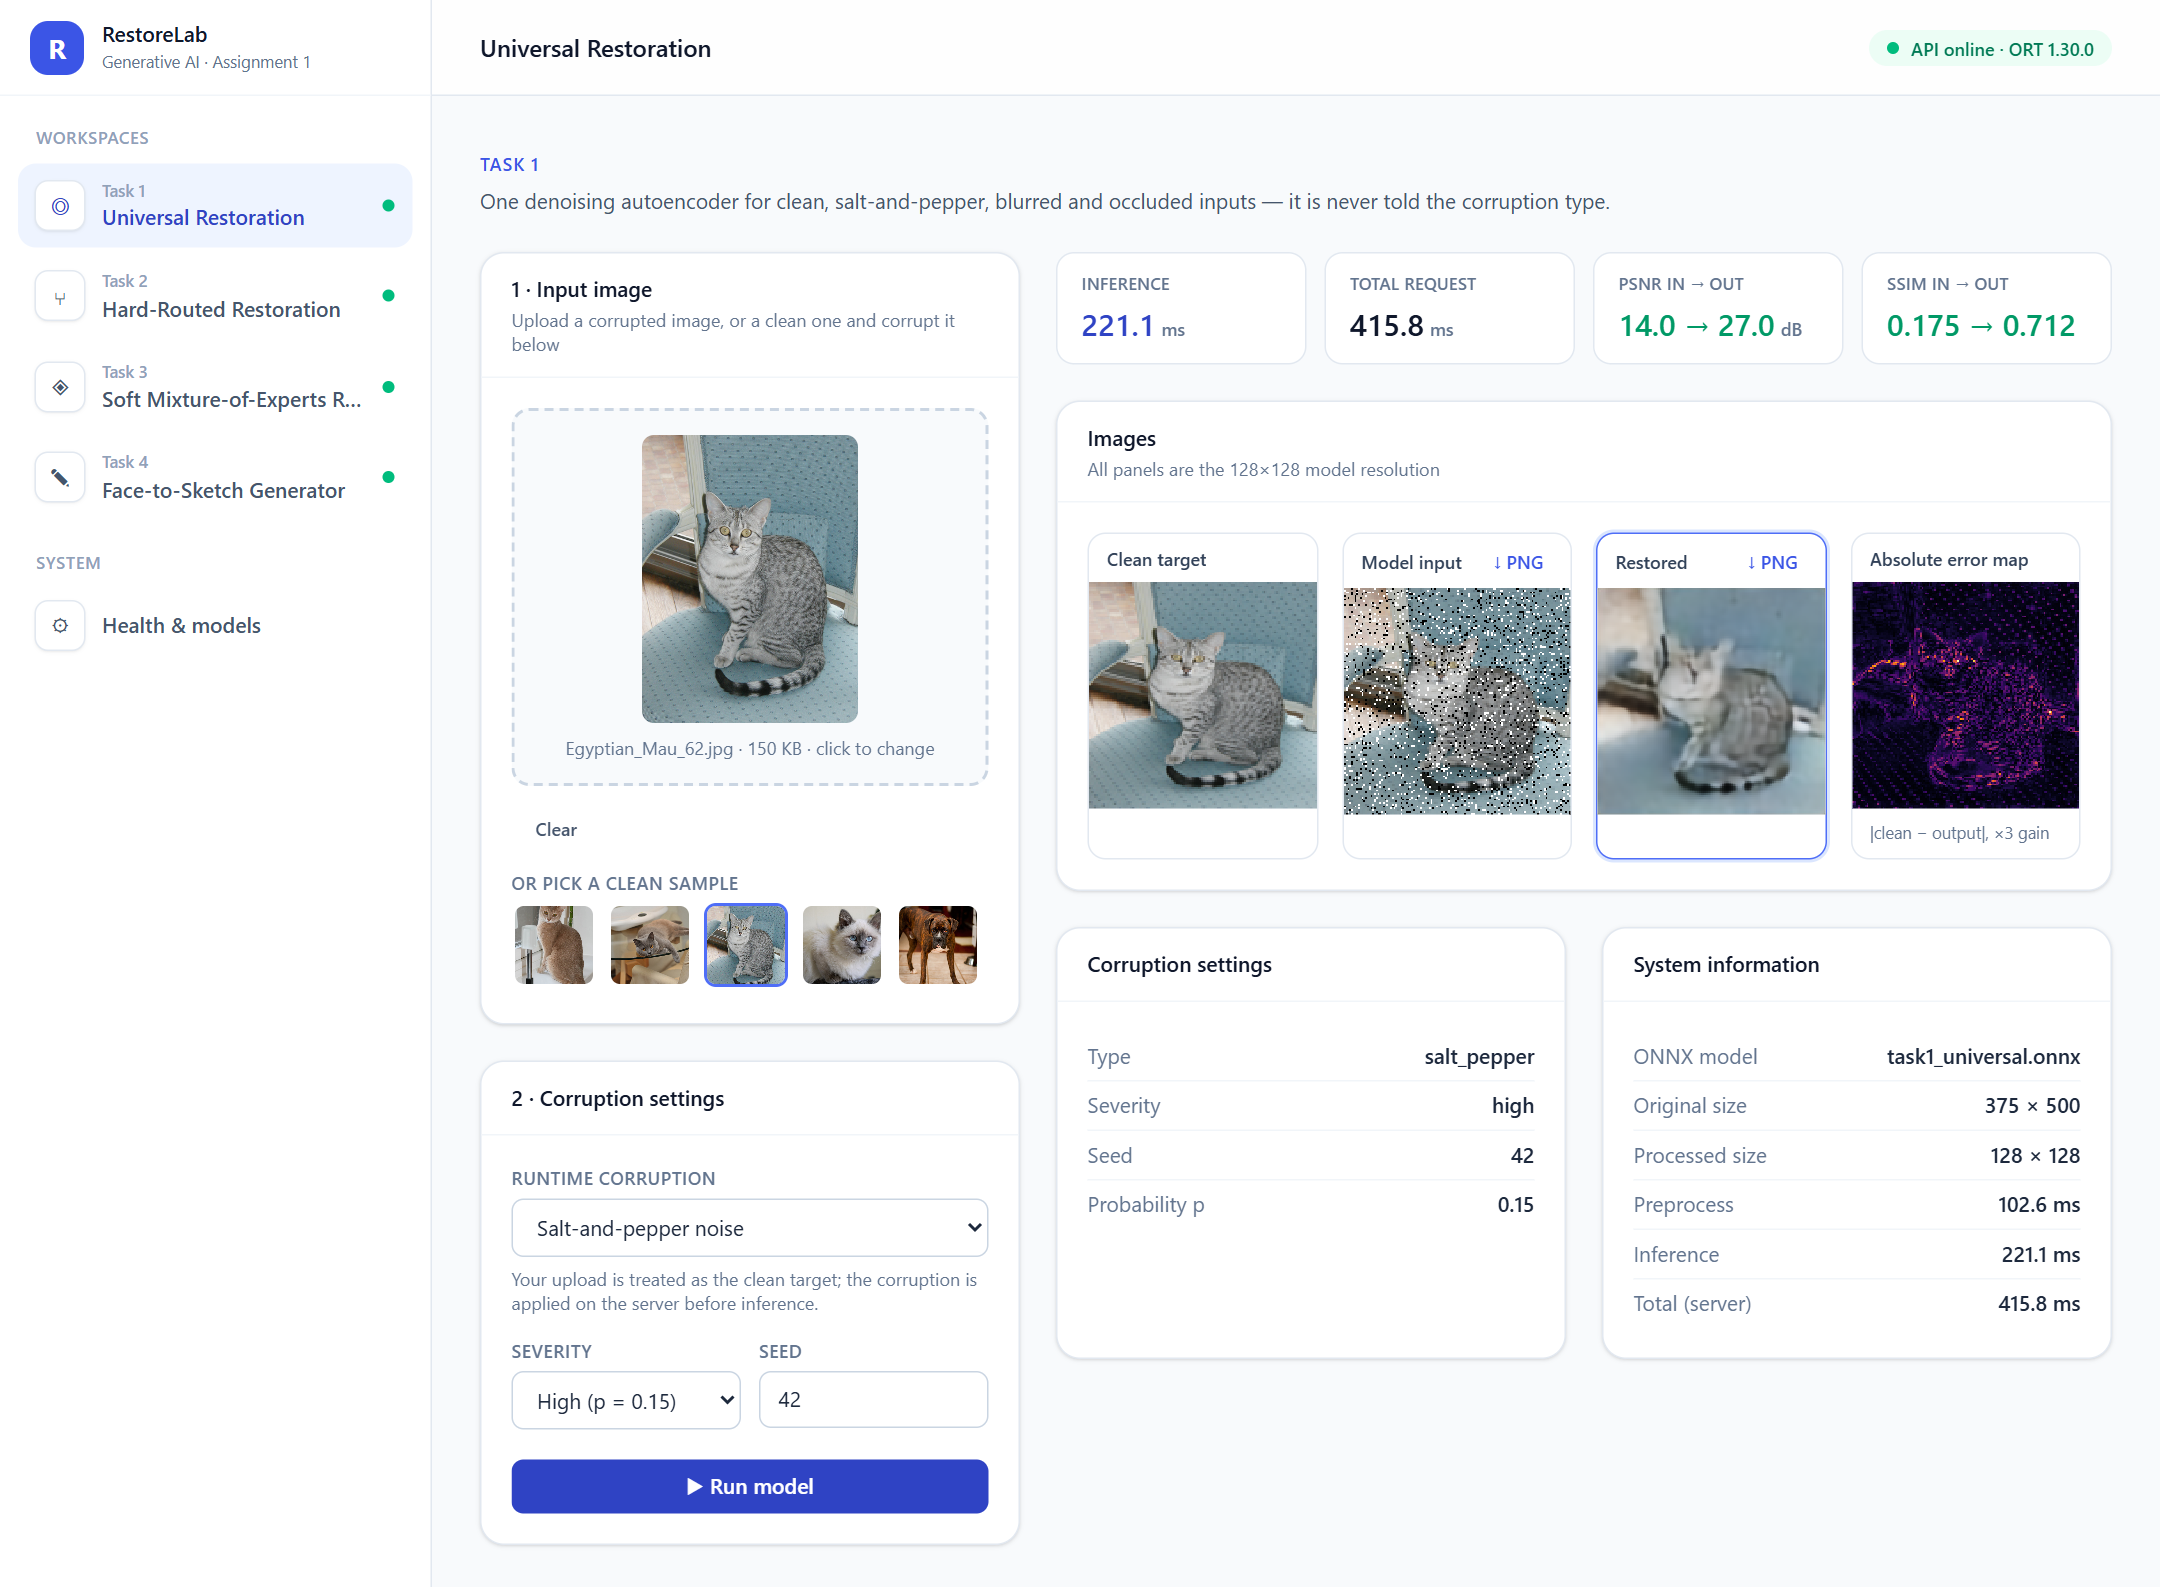
\includegraphics[width=0.49\textwidth]{app_shot_universal.png}\hfill
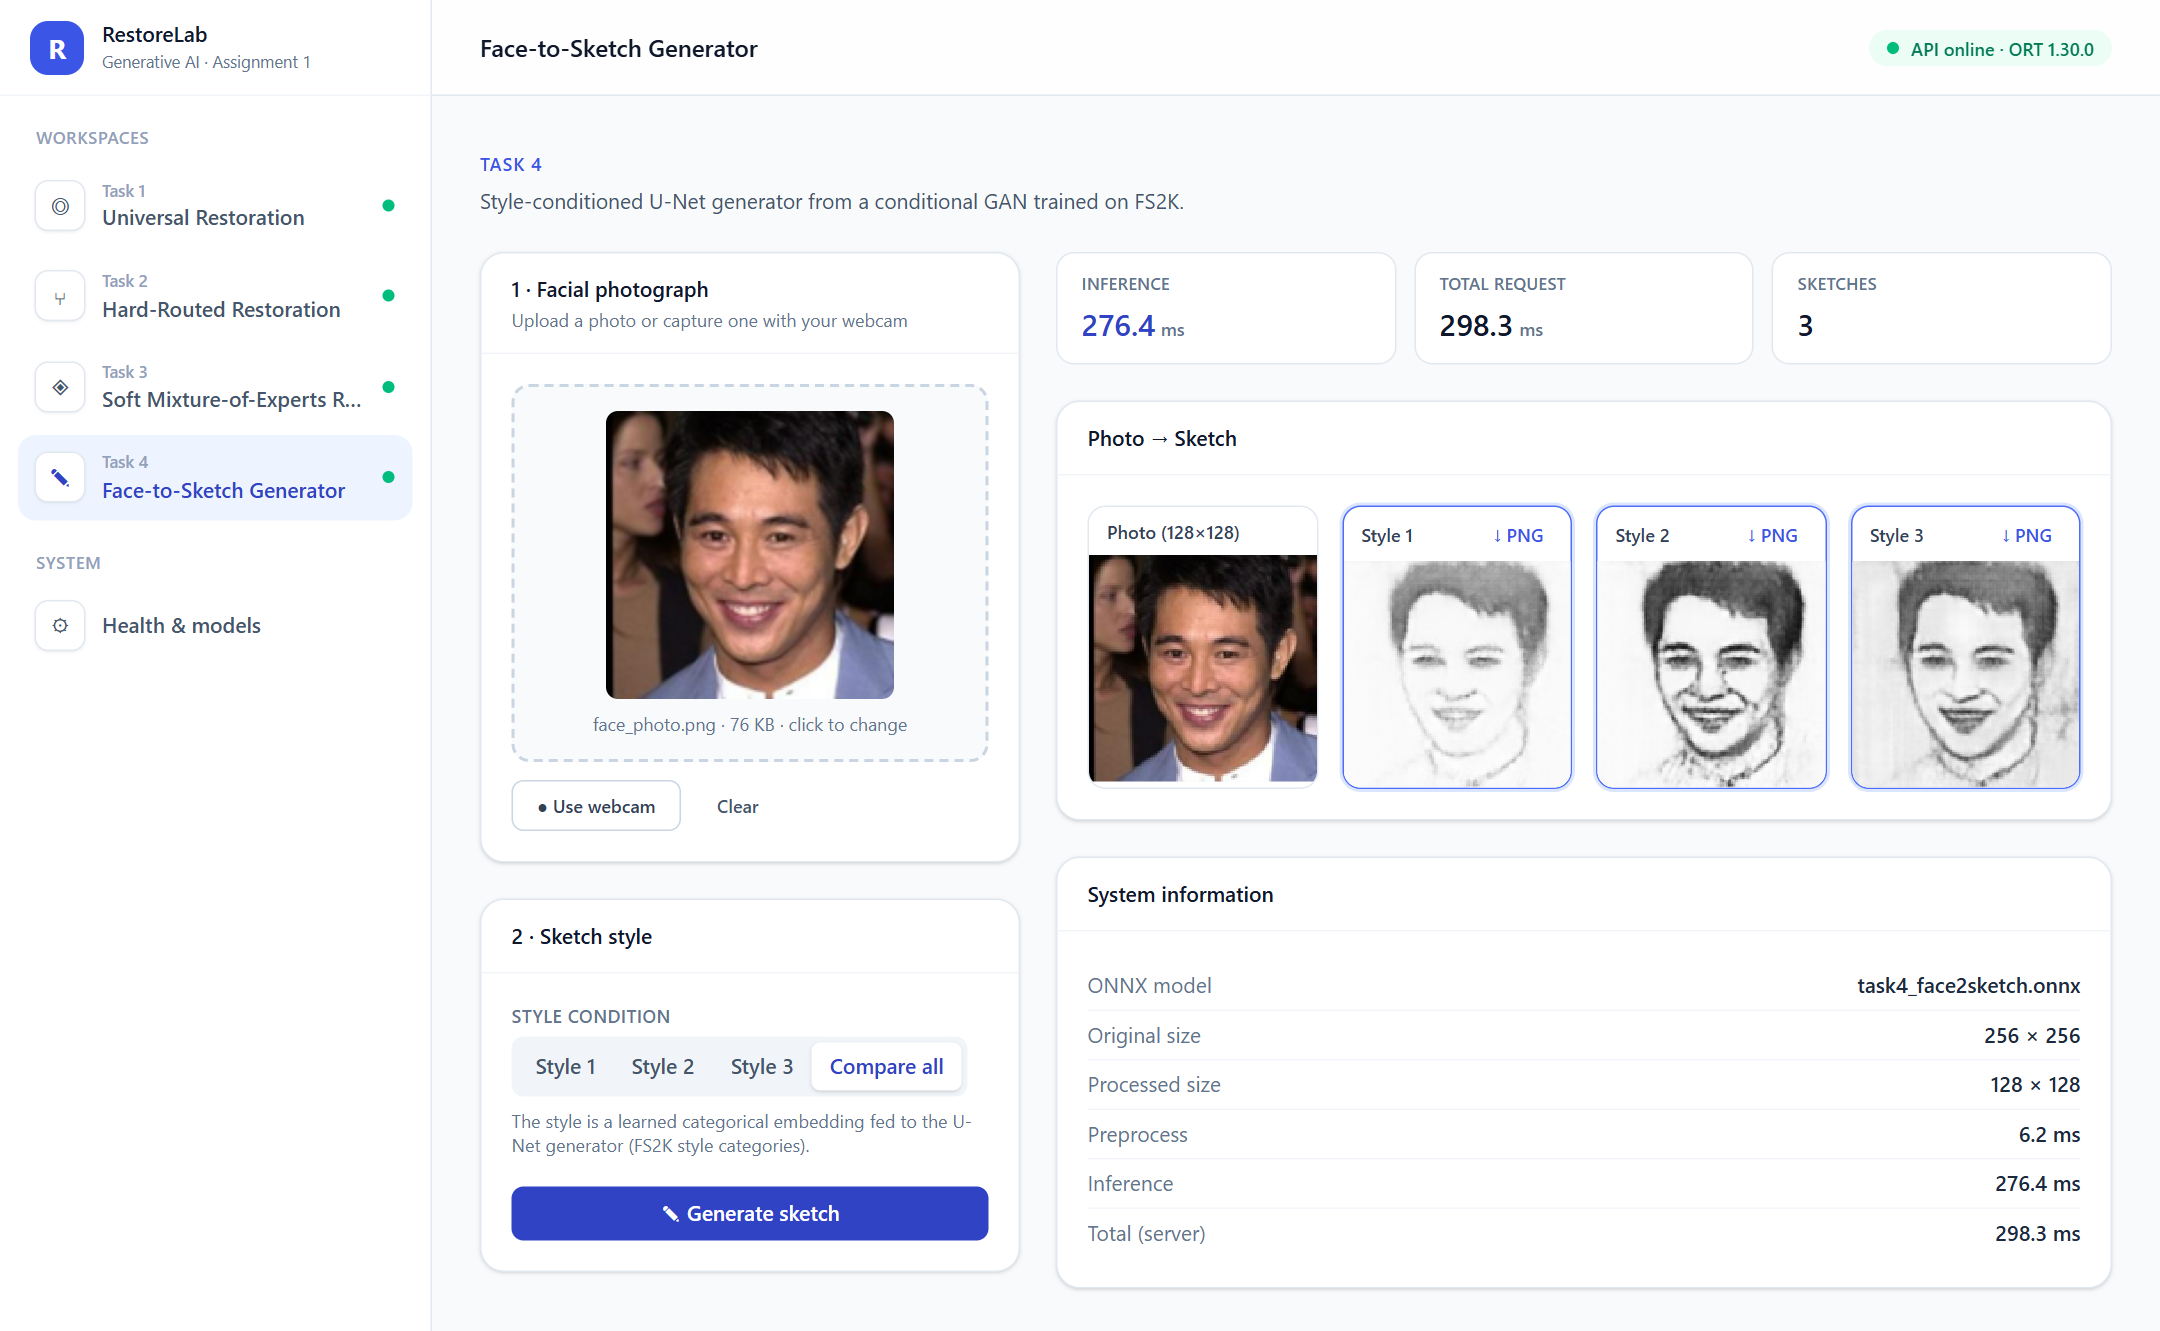
\includegraphics[width=0.49\textwidth]{app_shot_sketch.png}\\[2mm]
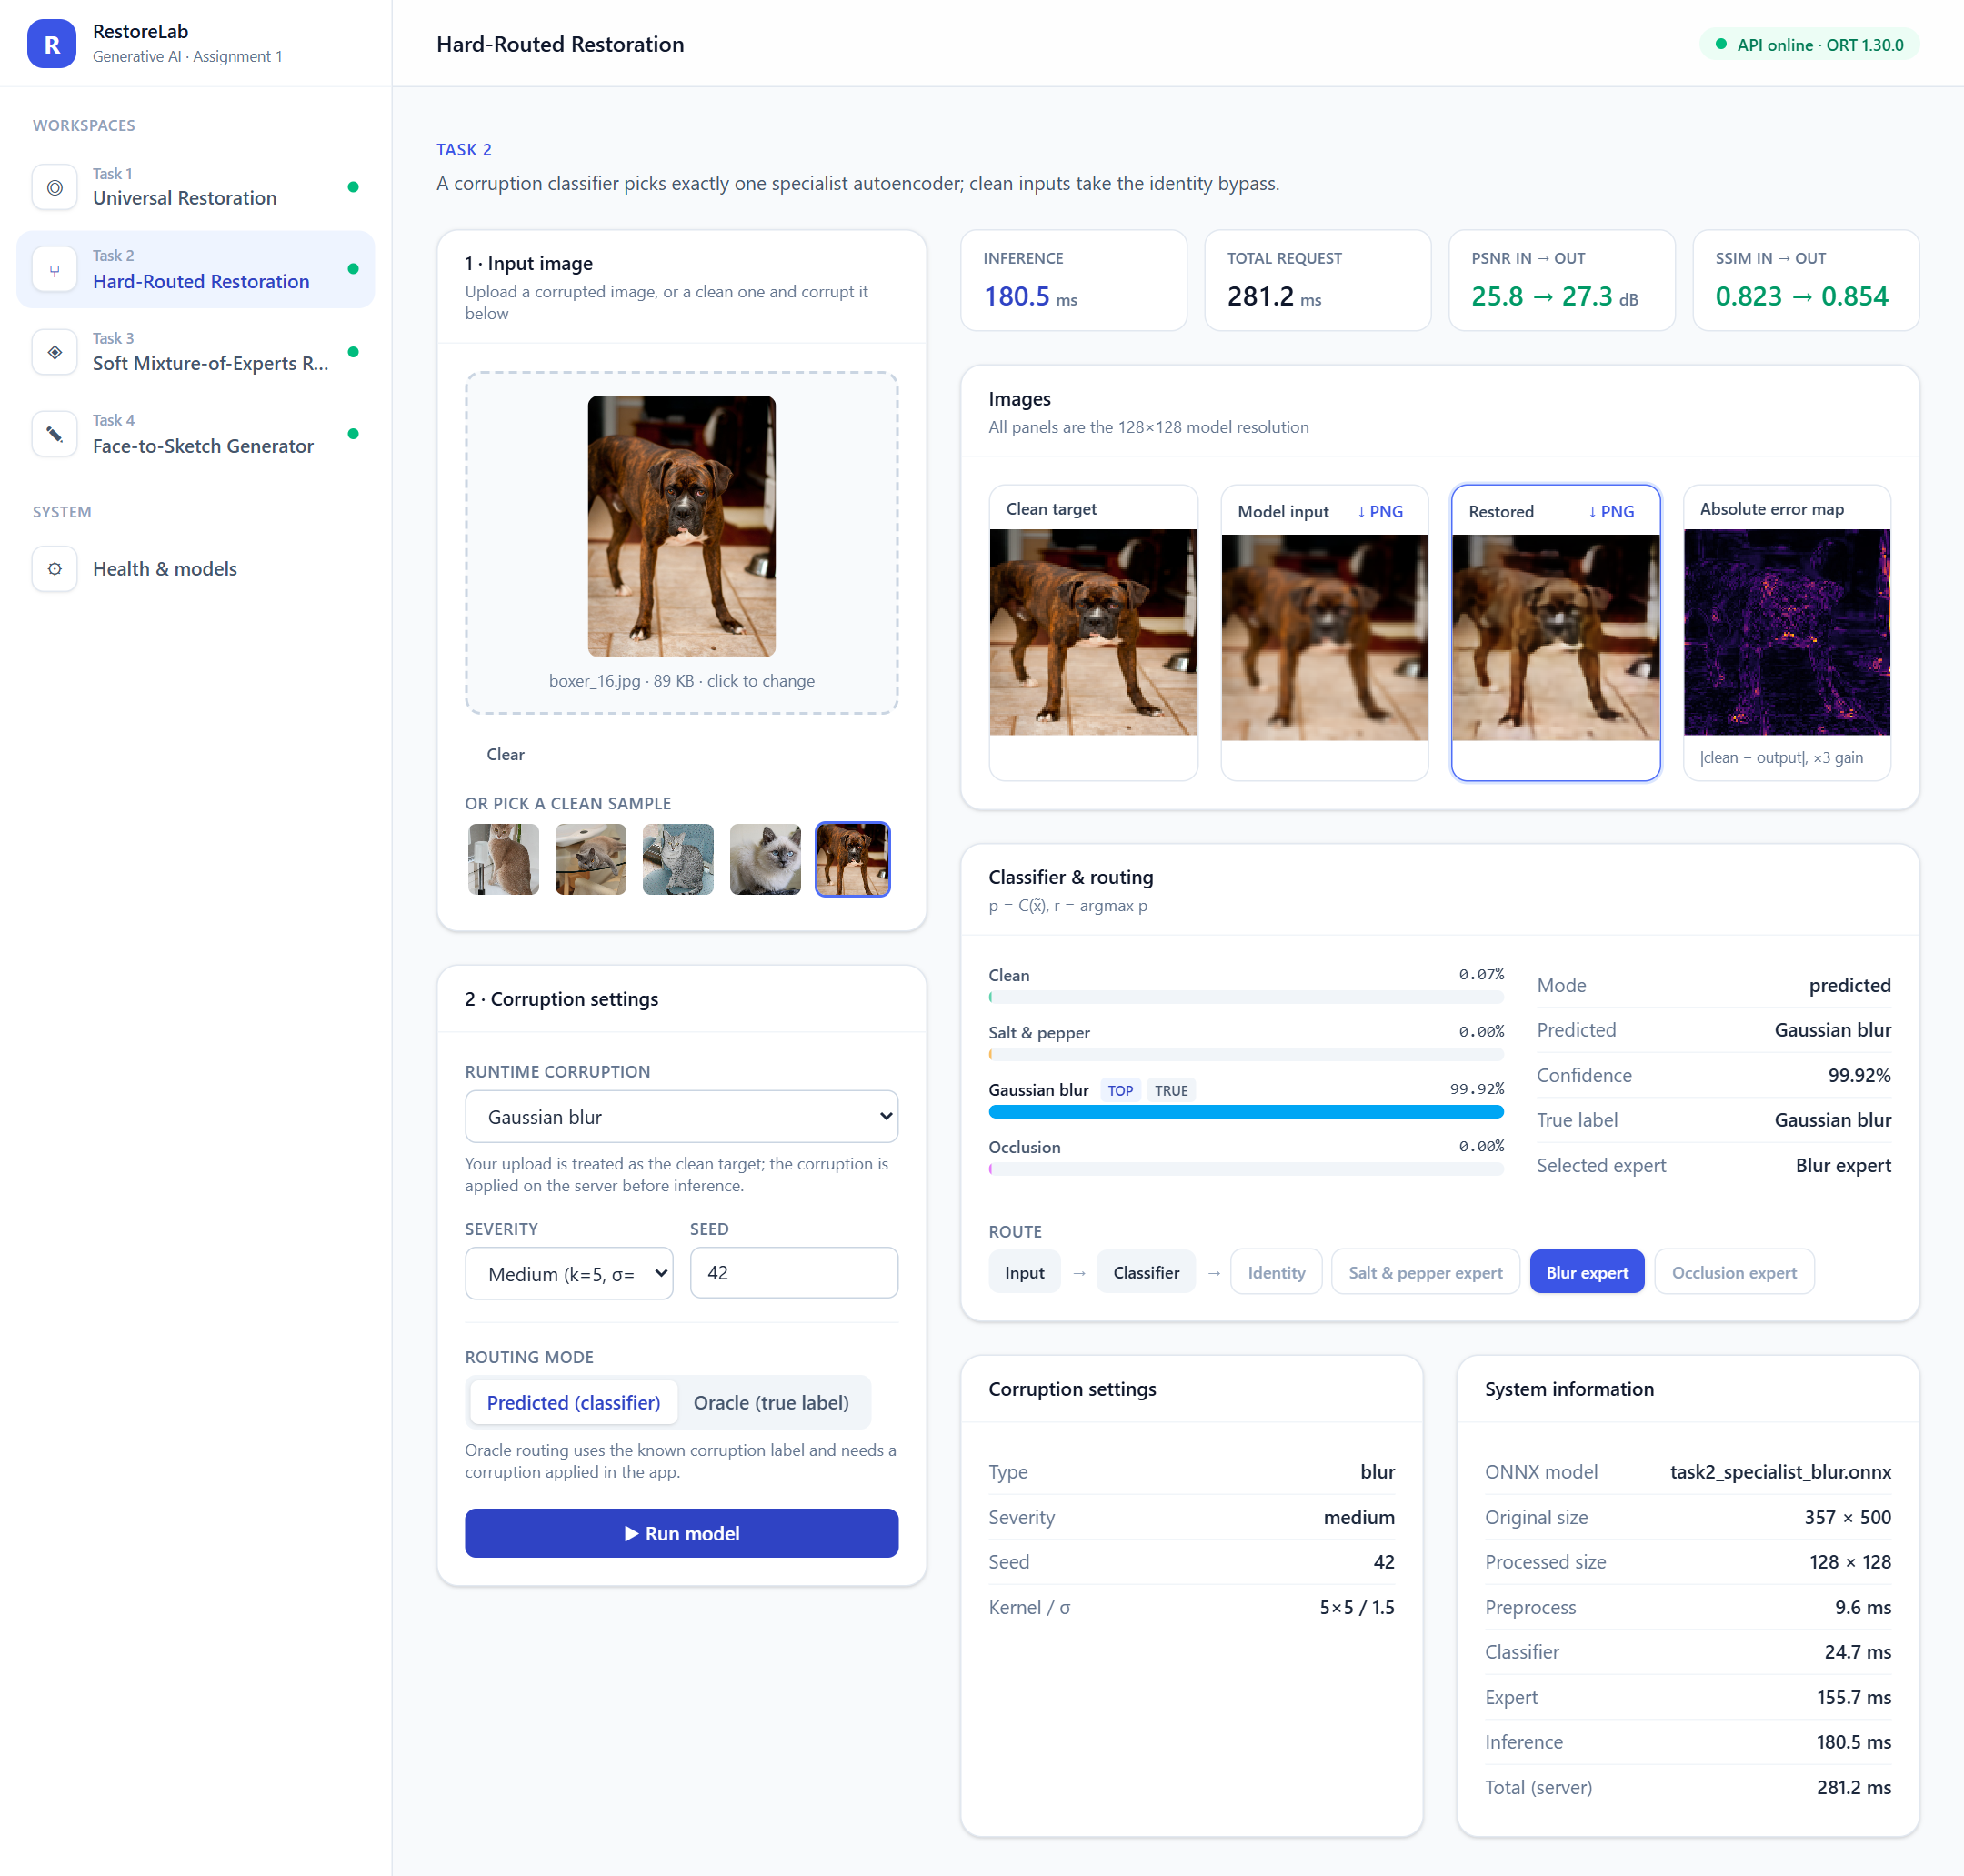
\includegraphics[width=0.49\textwidth]{app_shot_hard.png}\hfill
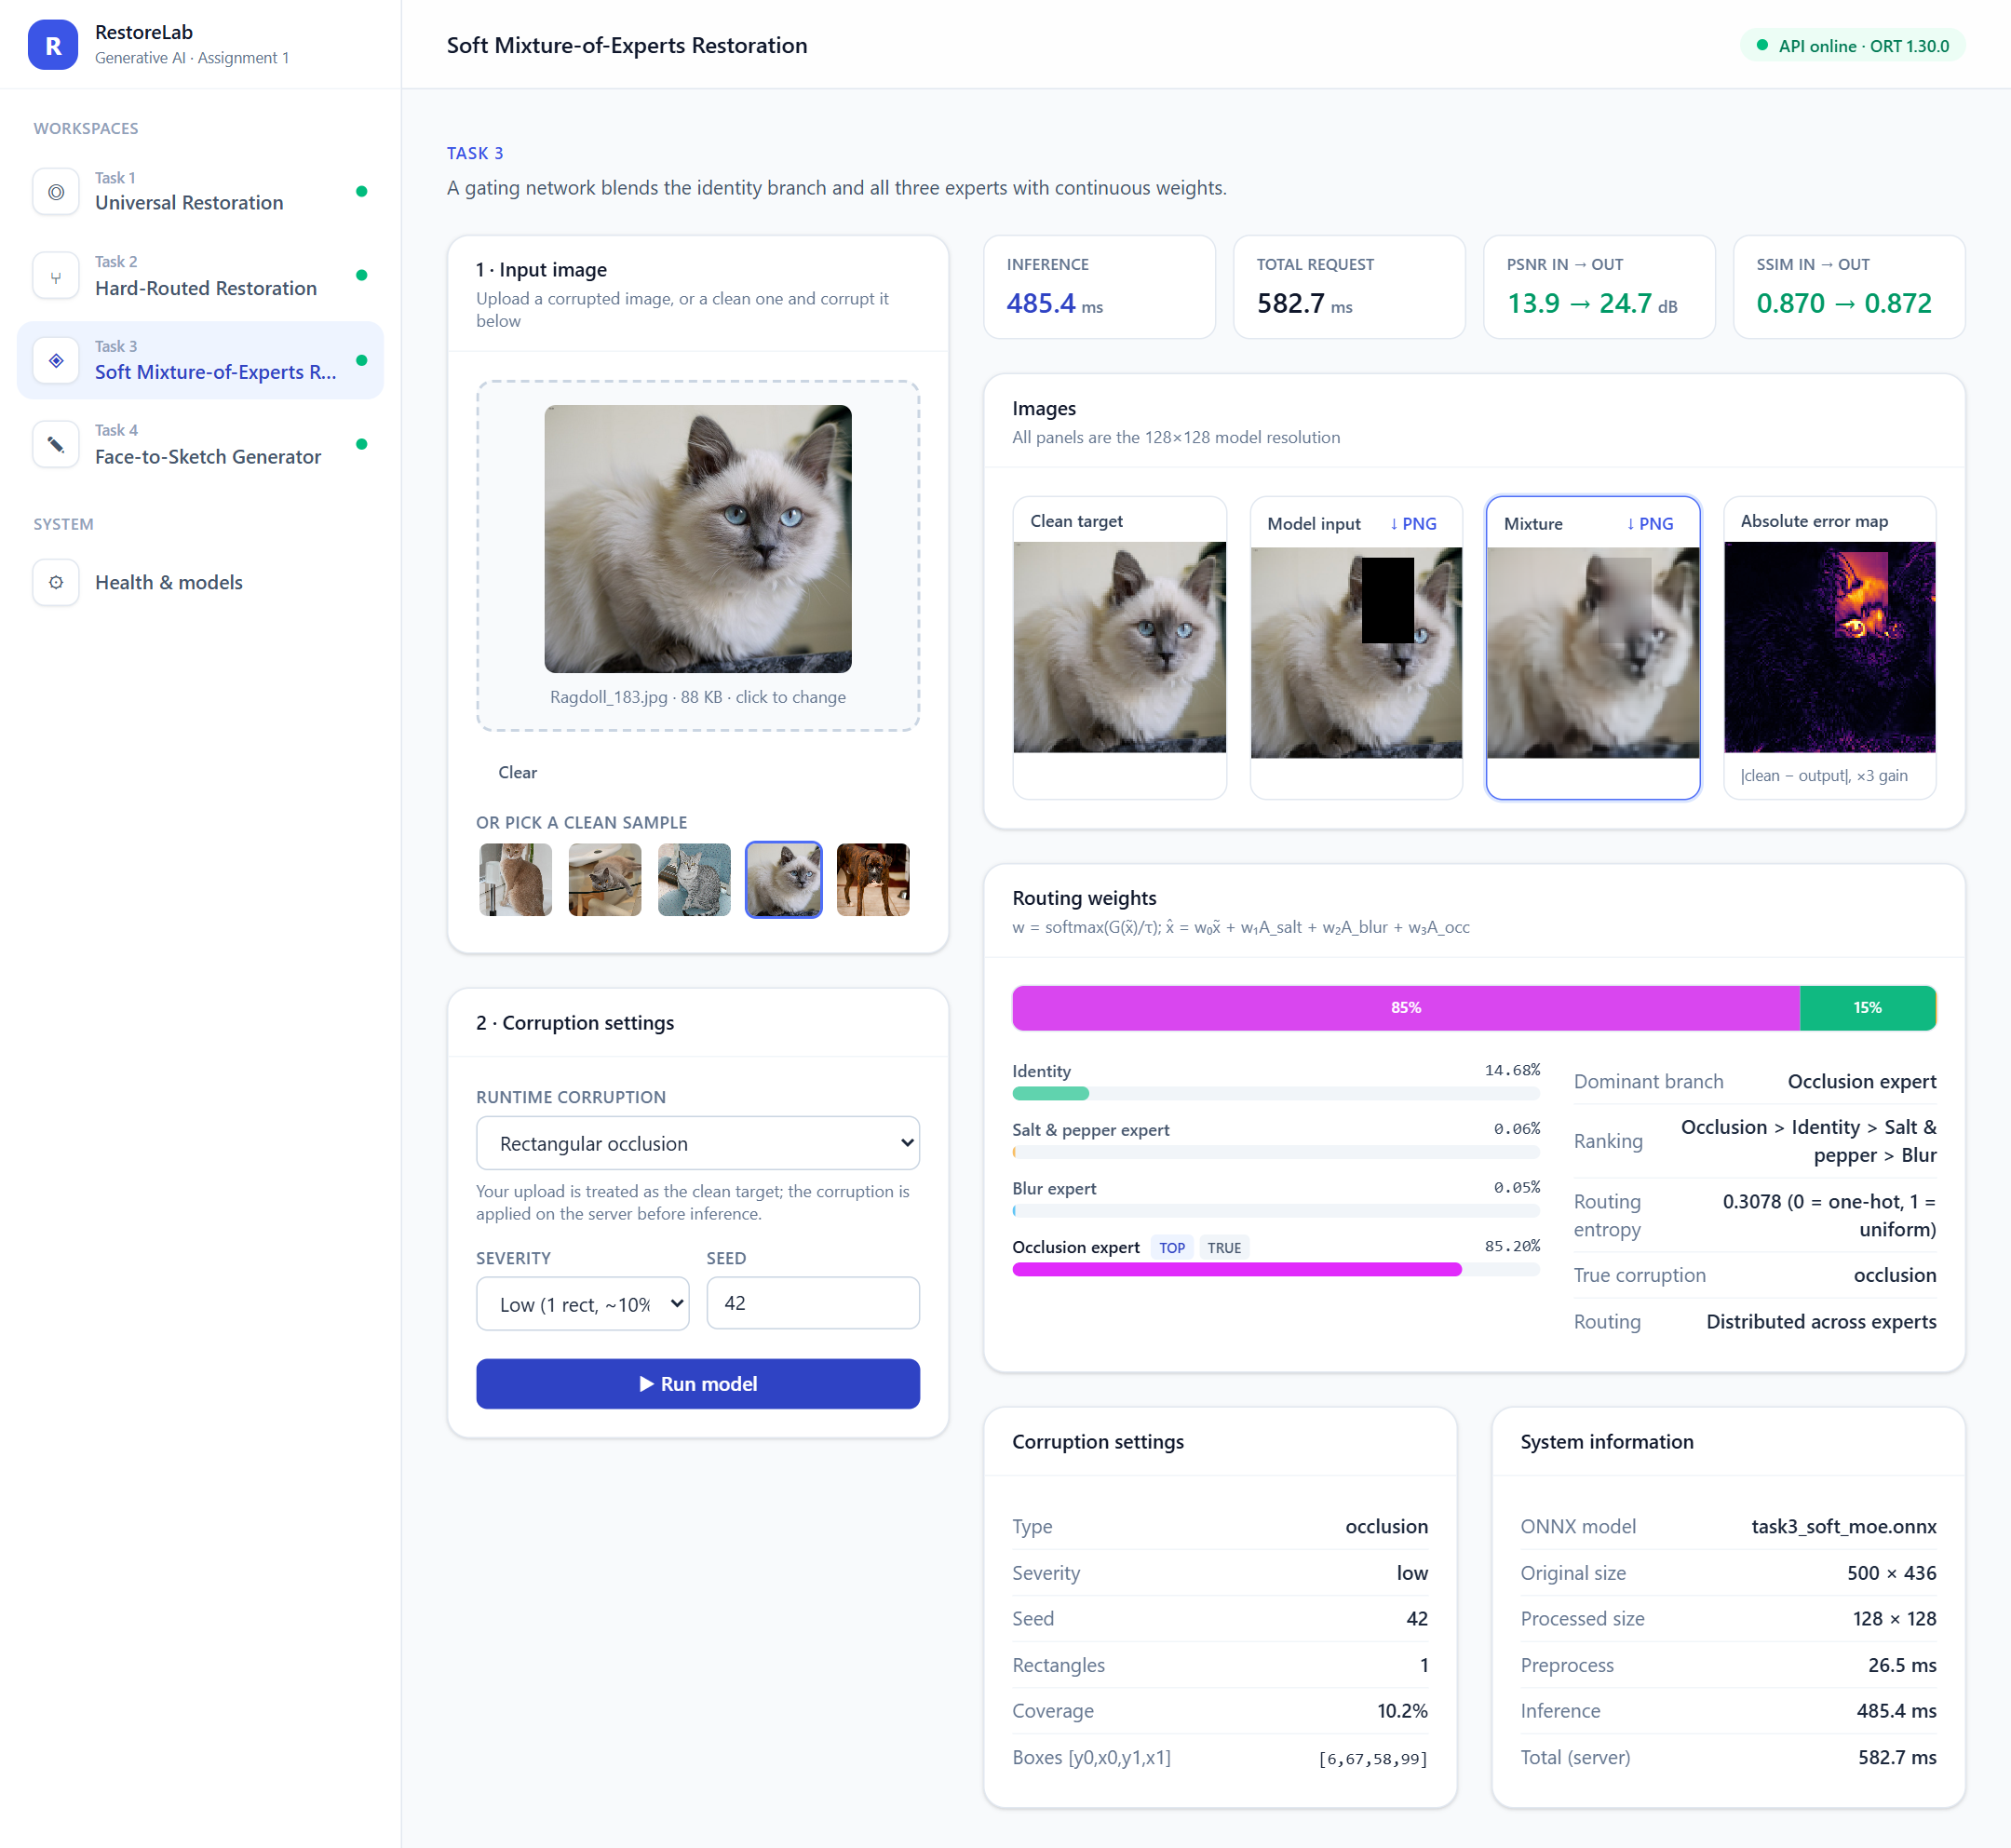
\includegraphics[width=0.49\textwidth]{app_shot_soft.png}
\caption{The running application with the trained ONNX models. Top left: Universal Restoration (salt-and-pepper, high: 13.5$\to$29.1\,dB). Top right: Face-to-Sketch Generator in all three styles. Bottom left: Hard-Routed Restoration (blur, 99.92\% confidence, blur expert selected). Bottom right: Soft Mixture-of-Experts on a low-severity occlusion, where the weight is split between the occlusion expert (85\%) and the identity branch (15\%).}
\label{fig:app}
\end{figure*}

\subsection{Containerised deployment}
The application consists of two containers started by Docker Compose (Fig.~\ref{fig:arch}). The backend image (\texttt{python:3.11-slim}) contains only FastAPI, ONNX Runtime, NumPy, OpenCV and Pillow, the API code and the corruption module, without PyTorch; it exposes a health check on \texttt{/api/health}. The frontend image is a multi-stage build: Node compiles the React app, and \texttt{nginx} serves the static files and proxies \texttt{/api} to the backend, so the browser talks to a single origin. The frontend starts only after the backend is healthy. The ONNX models (about 364\,MB in total) and the sample images are mounted read-only from the host (\texttt{./src/models}, \texttt{./backend/samples}), so updating a model needs a container restart but no rebuild. After cloning the repository and placing the model files in \texttt{src/models}, the complete application starts with \texttt{docker compose up --build} and is available at \texttt{http://localhost:8080}. Inside the container on a laptop CPU a request took about 0.2--0.4\,s end to end. The source code is at \url{\repourl}.\ifx\videourl\empty\else{} The demonstration video is at \url{\videourl}.\fi

\begin{figure}[t]
\centering
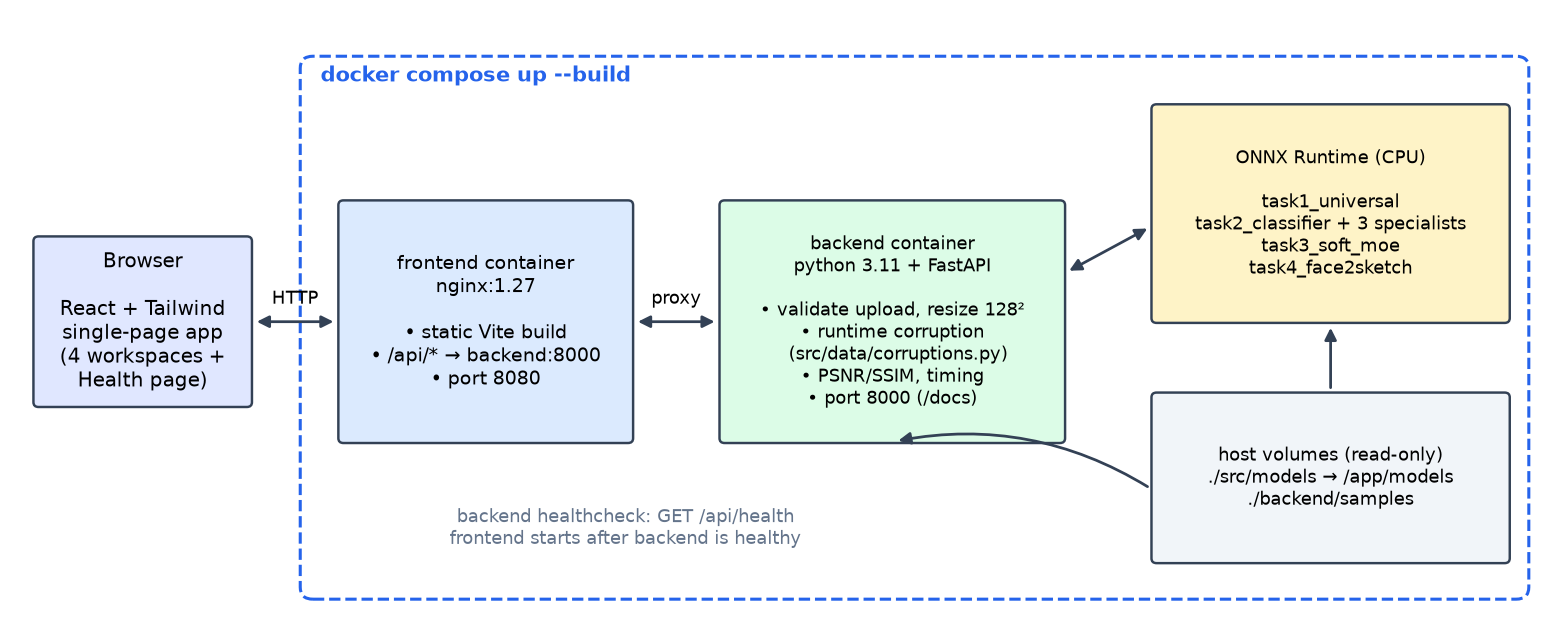
\includegraphics[width=\columnwidth]{app_architecture.png}
\caption{System architecture: browser, nginx frontend container, FastAPI backend container with ONNX Runtime, and model files mounted from the host.}
\label{fig:arch}
\end{figure}

% =====================================================================
\section{Discussion and Decisions}\label{sec:discussion}
The most important technical lessons were: (1) \emph{bottleneck shape beats bottleneck size}: the flat latent hit a $\approx$18\,dB wall at every size, while a spatial latent of comparable size reached 25.8\,dB; (2) \emph{a strong classifier makes both routing schemes equivalent}: with 99.8\% accurate routing, soft and hard routing differ by under 0.2\,dB on average; (3) \emph{mixtures of outputs cannot compose experts}: the universal model wins on mixed corruptions; (4) \emph{routing errors are explainable}: letterbox bars look like occlusion, and missed occlusions lie on dark regions where they do no harm; (5) \emph{a conditional label can be tested}: the style-swap table checks that the embedding is used.

\textbf{Limitations.} Several optima lie at the edge of their search ranges (Task 1 and Task 2 latent channels, base channels); Optuna studies have few completed trials, so importances are indicative; the classifier objective saturated; validation sets per corruption are small ($\approx$180); Task 4 uses 128-pixel images and pixel metrics; the final test evaluations of Tasks 1--3 were completed, but Task 4 is reported on the validation set only; no limited-skip-connection ablation was run; the application is deployed locally through Docker Compose and is not publicly hosted.

% =====================================================================
\section{Conclusion}
We built and evaluated four restoration and generation systems on shared infrastructure. A convolutional bottleneck was essential for restoration quality; hard routing with an identity bypass is a cheap, accurate improvement over the universal model for single corruptions; soft routing added cost without a PSNR benefit on the tested data; and the cGAN respects its style condition. All inference models run in ONNX Runtime behind one containerised web application that an evaluator can start with a single command and use on unseen images. Future work: training with compound corruptions and cascaded experts, a limited skip-connection ablation, a confidence threshold for routing, the official-test evaluation of the cGAN, and perceptual metrics for sketches.

% =====================================================================
\appendices
\section{Use of AI Tools}
\textbf{Tools:} Anthropic's Claude (chat interface and Claude Code in the development environment) and the AI features of Google Stitch. \textbf{Tasks:} literature suggestions, designing the experiment plan, writing and debugging the data pipeline, models, training, evaluation and export scripts, the FastAPI backend, the React frontend, the Dockerfiles and Compose configuration, the report-figure script, and drafting this report's text and \LaTeX; Google Stitch was used to generate and iterate on the interface design. \textbf{Verification:} every generated component was run and checked against measurements before being relied on. Examples of outputs that were tested and corrected: (i) the first MLflow setup failed on the current MLflow version (the file store is disabled), so the code was switched to a SQLite backend; (ii) a unit test exposed the overlapping-occlusion coverage bug (Section~III); (iii) the flat autoencoder's measured 18\,dB plateau led to the spatial bottleneck; (iv) the classifier's expected failure on mild blur did not occur, and the Optuna objective saturated, which was reported rather than hidden; (v) ONNX outputs were compared with PyTorch for several batch sizes and styles, and the routed pipeline was compared end-to-end; (vi) the backend was tested with dummy ONNX models and then with the real models in Docker, which exposed and fixed a non-JSON-compliant infinite PSNR for unchanged clean inputs; (vii) the draft hypothesis about missed occlusions was checked against the per-sample test data before being stated. I can explain and modify every submitted component.

\section{Decision Log}
Table~\ref{tab:log} lists the decisions in chronological order.

\begin{table*}[t]
\caption{Chronological decisions, reasons and evidence.}
\label{tab:log}
\centering\footnotesize
\begin{tabular}{@{}lp{6.4cm}p{8.6cm}@{}}
\toprule
Stage & Decision & Reason / evidence\\
\midrule
Data & Single JSON ``condition'' per corruption; runtime training corruption; stored val/test manifests & Required by the brief; makes validation/test reproducible and shares code with the web app\\
Data & Overlap-avoiding box placement & Unit test: coverage of the 35\% setting was only $\approx$30\%; now 34.9\%\\
Tooling & MLflow with SQLite; Optuna with SQLite & New MLflow disables the file store; SQLite lets Optuna resume after session loss\\
Tooling & Test set guarded by a \texttt{--final} flag; each evaluation run once & Brief: test set untouched until final evaluation\\
Tooling & Zip and download after every stage & A Kaggle session was wiped once and work was lost\\
T1 & Objective $S=0.5\,\mathrm{SSIM}+0.5\min(\mathrm{PSNR},40)/40$ & Combines fidelity and structure; independent of $\alpha$ so trials are comparable\\
T1 & Widened latent range to 4096 after the baseline & Baseline showed a bottleneck-limited model (18\,dB, train $\approx$ val loss)\\
T1 & Replaced the flat latent by an $8{\times}8{\times}C$ bottleneck & Latent size had importance 0.004; flat model at 18.8\,dB after tuning; spatial reached 25.8\,dB\\
T1 & No skip connections & Guarantees a true bottleneck; limited-skip ablation left for future work\\
T2 & Exactly balanced batches; no early down-sampling; macro-F1 objective & Brief requires balance; fine pixel cues; avoids majority-class bias\\
T2 & Kept trial \#4 although the objective saturated & Ties could not be broken on validation; reported as a limitation\\
T2 & One shared Optuna search on a 3-type mixture; three independent trainings with different seeds & Allowed by the brief and affordable; separate parameters guaranteed\\
T2 & Identity bypass for clean & Task 1: restoration reduces quality of clean/mild inputs ($50\to27$\,dB)\\
T3 & Gate and experts initialised from Task 2; 3-epoch warm-up; frozen experts in eval mode & Required; avoids random routing and BatchNorm drift\\
T3 & Balance loss as in the brief, collapse pruning, 25\% epochs & Prevents expert collapse; keeps trials affordable\\
T3 & Reported the negative mixed-corruption result & Gate was near one-hot; universal model better; explained by convex output blending\\
T4 & Stratified 15\% validation, official test untouched & Brief; style counts balanced in train/val\\
T4 & Style embedding via input concatenation plus FiLM in the decoder; embedding also in the discriminator & Brief: not just an interface label; FiLM conditions every decoder level\\
T4 & Objective SSIM$-\ell_1$; style-swap test & Cheap proxy for GAN quality; checks that the condition is used\\
Export & ONNX wrappers: softmax inside classifier, scaling inside generator, pipeline check & Simplifies the application; verified on several batch sizes\\
App & ONNX Runtime on CPU; missing model $\to$ HTTP 503; tests with dummy models & Runs in Docker without GPU; kept the app usable while Task 4 trained\\
App & nginx serves the build and proxies \texttt{/api}; models mounted read-only & One origin for the browser (no CORS); models updated without rebuilding images\\
\bottomrule
\end{tabular}
\end{table*}

% =====================================================================
\begin{thebibliography}{99}
\bibitem{vincent2008} P.~Vincent, H.~Larochelle, Y.~Bengio and P.-A.~Manzagol, ``Extracting and composing robust features with denoising autoencoders,'' in \emph{Proc. ICML}, 2008.
\bibitem{wang2004} Z.~Wang, A.~C.~Bovik, H.~R.~Sheikh and E.~P.~Simoncelli, ``Image quality assessment: from error visibility to structural similarity,'' \emph{IEEE Trans. Image Process.}, vol.~13, no.~4, pp.~600--612, 2004.
\bibitem{zhao2017} H.~Zhao, O.~Gallo, I.~Frosio and J.~Kautz, ``Loss functions for image restoration with neural networks,'' \emph{IEEE Trans. Comput. Imaging}, vol.~3, no.~1, pp.~47--57, 2017.
\bibitem{jacobs1991} R.~A.~Jacobs, M.~I.~Jordan, S.~J.~Nowlan and G.~E.~Hinton, ``Adaptive mixtures of local experts,'' \emph{Neural Comput.}, vol.~3, no.~1, pp.~79--87, 1991.
\bibitem{shazeer2017} N.~Shazeer \emph{et al.}, ``Outrageously large neural networks: the sparsely-gated mixture-of-experts layer,'' in \emph{Proc. ICLR}, 2017.
\bibitem{fedus2022} W.~Fedus, B.~Zoph and N.~Shazeer, ``Switch Transformers: scaling to trillion parameter models with simple and efficient sparsity,'' \emph{J. Mach. Learn. Res.}, vol.~23, 2022.
\bibitem{goodfellow2014} I.~Goodfellow \emph{et al.}, ``Generative adversarial nets,'' in \emph{Proc. NeurIPS}, 2014.
\bibitem{mirza2014} M.~Mirza and S.~Osindero, ``Conditional generative adversarial nets,'' arXiv:1411.1784, 2014.
\bibitem{ronneberger2015} O.~Ronneberger, P.~Fischer and T.~Brox, ``U-Net: convolutional networks for biomedical image segmentation,'' in \emph{Proc. MICCAI}, 2015.
\bibitem{isola2017} P.~Isola, J.-Y.~Zhu, T.~Zhou and A.~A.~Efros, ``Image-to-image translation with conditional adversarial networks,'' in \emph{Proc. CVPR}, 2017.
\bibitem{perez2018} E.~Perez, F.~Strub, H.~de~Vries, V.~Dumoulin and A.~Courville, ``FiLM: visual reasoning with a general conditioning layer,'' in \emph{Proc. AAAI}, 2018.
\bibitem{miyato2018} T.~Miyato and M.~Koyama, ``cGANs with projection discriminator,'' in \emph{Proc. ICLR}, 2018.
\bibitem{akiba2019} T.~Akiba, S.~Sano, T.~Yanase, T.~Ohta and M.~Koyama, ``Optuna: a next-generation hyperparameter optimization framework,'' in \emph{Proc. KDD}, 2019.
\bibitem{loshchilov2019} I.~Loshchilov and F.~Hutter, ``Decoupled weight decay regularization,'' in \emph{Proc. ICLR}, 2019.
\bibitem{parkhi2012} O.~M.~Parkhi, A.~Vedaldi, A.~Zisserman and C.~V.~Jawahar, ``Cats and dogs,'' in \emph{Proc. CVPR}, 2012.
\bibitem{fan2022} D.-P.~Fan, Z.~Huang, P.~Zheng, H.~Liu, X.~Qin and L.~Van~Gool, ``Facial-sketch synthesis: a new challenge,'' \emph{Mach. Intell. Res.}, vol.~19, no.~4, pp.~257--287, 2022.
\end{thebibliography}

\end{document}
